% \meutodo{
%   Variação gradual de parâmetros para identificar o que causa perdas/ganhos
% }

%%%%%%%%%%%%%%%%%%%%%%%%%%%%%%%%%%%%%%%%%%%%%%%%%%%%%%%%%%%%%%%%%%%%%%%%%%%%%%%%
\section{Considerações Iniciais}

Este capítulo apresenta os resultados encontrados quando os métodos de processamento descritos nos capítulos anteriores foram aplicados no pipeline de reconhecimento de imagens. Para cada experimento realizado, são descritos: a base de imagens, o protocolo utilizado, os resultados encontrados e a discussão da relevância de tais resultados.

Primeiramente os experimentos são relacionados à \textbf{quantização} de imagens e posteriormente à \textbf{geração de imagens} para rebalancear classes. Ambos processamentos são realizados antes da extração de características, e portanto no campo visual. Por conta disso, os resultados devem refletir melhoras nas etapas subsequentes, como uma melhor acurácia na etapa de classificação ou a redução do tempo de processamento.

%%%%%%%%%%%%%%%%%%%%%%%%%%%%%%%%%%%%%%%%%%%%%%%%%%%%%%%%%%%%%%%%%%%%%%%%%%%%%%%%
\section{Quantização de Imagens}

O objetivo dessa seção é mostrar os efeitos da etapa de quantização e como ela pode ser utilizada para reduzir a dimensionalidade do espaço de características. A Figura \ref{fig:quant:flowResult} demonstra o fluxo das operações e os métodos utilizados nos experimentos. Inicialmente, as imagens foram quantizadas em 256, 128, 64, 32 e 16 cores. Após, suas características foram extraídas e duas etapas de experimentos são realizadas:

\begin{enumerate}
  \item Experimentos utilizando um método de extração de características seguido pela classificação (sem posterior seleção de características);
  \item Experimentos utilizando o vetor resultante da concatenação de todos os métodos de extração, seguido pela classificação com e sem a seleção de características.
\end{enumerate}

\begin{figure}[htbp]
  \begin{center}
    \centering
    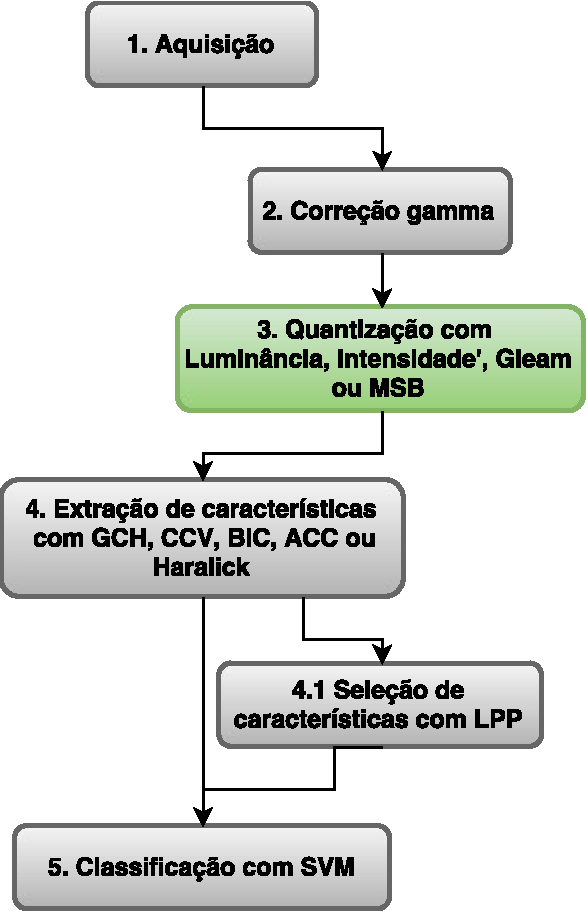
\includegraphics[width=0.4\linewidth]{\detokenize{figuras/quantizacao/quantizationResult.pdf}}
  \end{center}
  \caption[Essa figura demonstra o fluxo das operações e os métodos utilizados nos experimentos. Após a aquisição da imagem, ela é convertida para escala de cinza por algum método de quantização e seus níveis de cor reduzidos por um parâmetro de quantização. Dependendo do método, a correção \emph{gamma} é realizada. A imagem quantizada serve então como entrada para um método de extração de características e posteriormente é classificada com \emph{SVM}. Uma das etapas de experimentos prevê também a concatenação de todos os vetores extraídos e a seleção das características com \emph{LPP} antes da classificação.]{Essa figura demonstra o fluxo das operações e os métodos utilizados nos experimentos. Após a aquisição da imagem, ela é convertida para escala de cinza por algum método de quantização e seus níveis de cor reduzidos por um parâmetro de quantização. Dependendo do método, a correção \emph{gamma} é realizada. A imagem quantizada serve então como entrada para um método de extração de características e posteriormente é classificada com \emph{SVM}. Uma das etapas de experimentos prevê também a concatenação de todos os vetores extraídos e a seleção das características com \emph{LPP} antes da classificação. \textit{Fonte:~Elaborado pela autora.}}
  \label{fig:quant:flowResult}
\end{figure}

%%%%%%%%%%%%%%%%%%%%%%%%%%%%%%%%%%%%%%%%%%%%%%%%%%%%%%%%%%%%%%%%%%%%%%%%%%%%%%%%
\subsection{Base de Imagens}

Três bases de imagens, ilustradas na Figura~\ref{fig:quant:bases}, foram utilizadas nestes experimentos:
\begin{itemize}
\item[] \textbf{Corel-1000}\footnote{Disponível em http://www.wang.ist.psu.edu/docs/related/}: consiste em dez classes balanceadas de imagens naturais, com algumas classes bem definidas e algumas não;
\item[] \textbf{Caltech101-600}\footnote{Disponível em http://www.vision.caltech.edu/ImageDatasets/Caltech101/}: contém fotos e desenhos. Desta base, foi utilizado um conjunto de seis classes balanceadas: aviões, bonsais, candelabros, tartarugas, motocicletas e relógios;
\item[] \textbf{Produce}\footnote{Disponível em ??} (também conhecido como base de vegetais e frutas tropicais): composta por imagens com um fundo similar mas muitas mudanças na iluminação, no número de objetos e na escala. Apesar da oclusão parcial de objetos ser observada, essa classe possui dados bem comportados.
\end{itemize}

\begin{figure}[htbp]
  \begin{center}
  \begin{subfigure}{.6\textwidth}
    \centering
    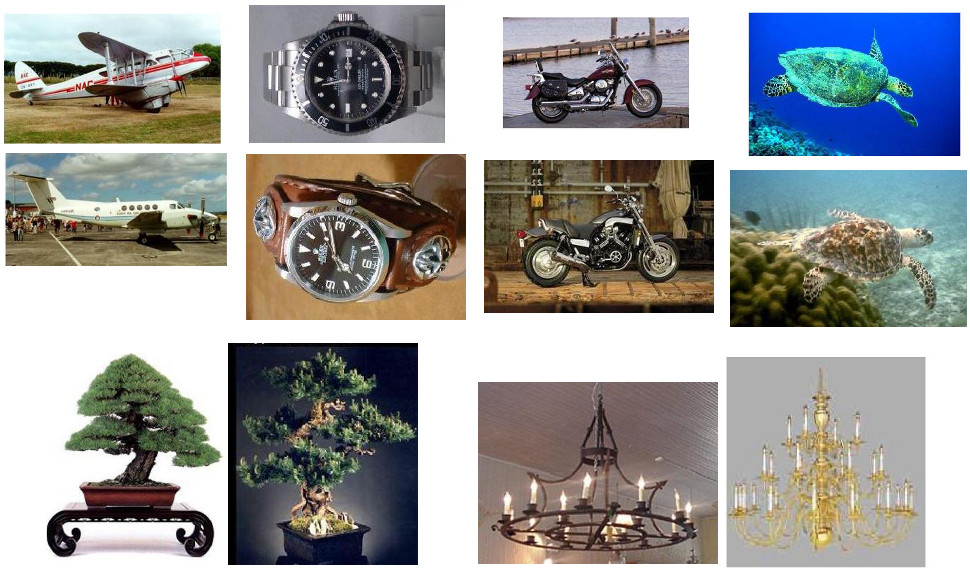
\includegraphics[width=\linewidth]{\detokenize{figuras/quantizacao/fig_Caltech101_dataset.jpg}}
    \caption{Base de imagens Caltech101}
  \end{subfigure}
  \begin{subfigure}{.6\textwidth}
    \centering
    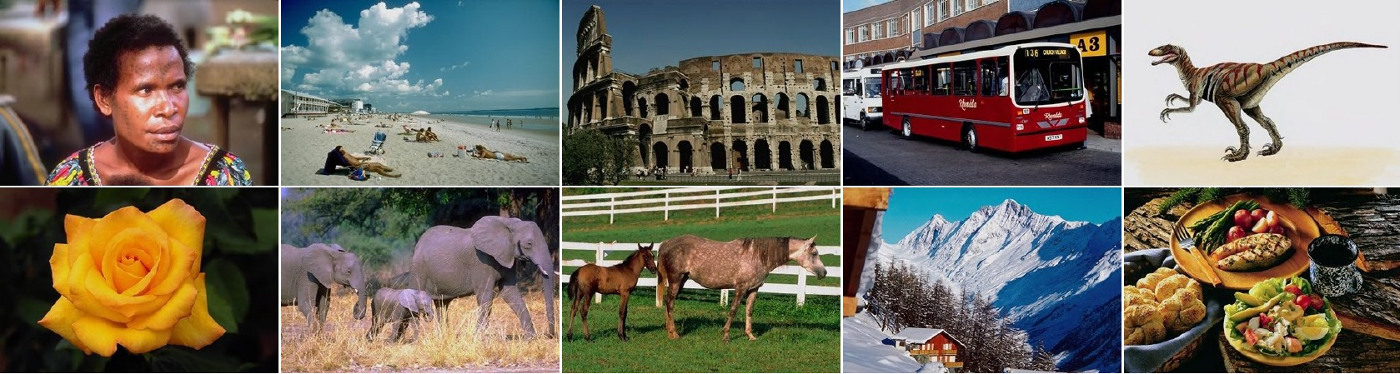
\includegraphics[width=\linewidth]{\detokenize{figuras/quantizacao/fig_COREL_dataset.jpg}}
    \caption{Base de imagens Corel-1000}
  \end{subfigure}
  \begin{subfigure}{.6\textwidth}
    \centering
    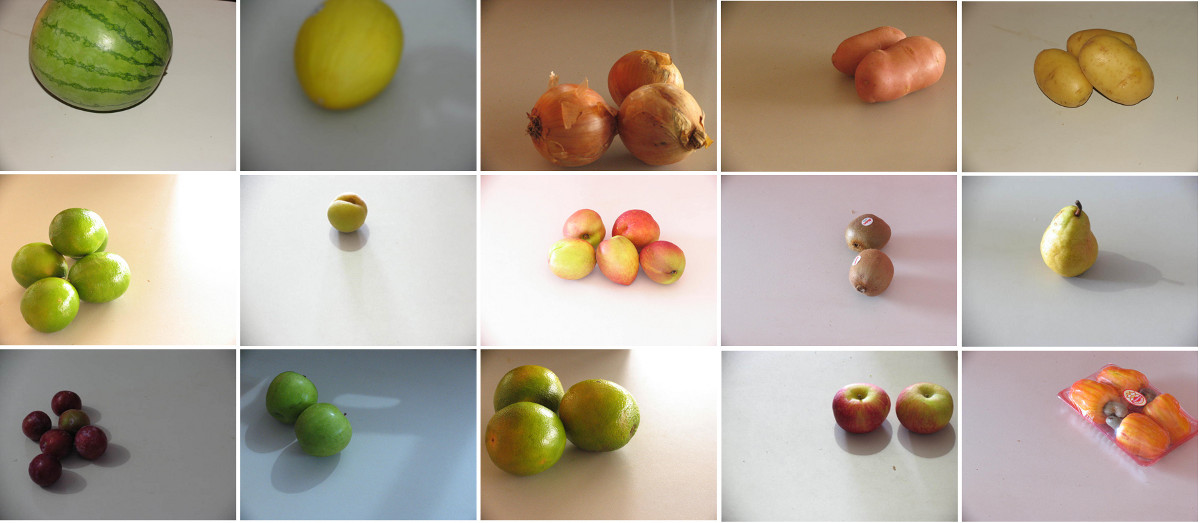
\includegraphics[width=\linewidth]{\detokenize{figuras/quantizacao/fig_Produce_dataset.jpg}}
    \caption{Base de imagens Produce}
  \end{subfigure}
  \end{center}
  \caption[Bases de imagens utilizadas para os experimentos de quantização.]{Bases de imagens utilizadas para os experimentos de quantização. \textit{Fonte:~\cite{Ponti2016}.}}
  \label{fig:quant:bases}
\end{figure}

Estes experimentos possuem foco na redução na dimensionalidade. Para evitar o problema do desbalanceamento, as bases \textit{Produce} e \textit{Caltech101} foram modificadas. Dessa forma, as classes disponíveis foram balanceadas ao remover imagens das classes majoritárias.

%%%%%%%%%%%%%%%%%%%%%%%%%%%%%%%%%%%%%%%%%%%%%%%%%%%%%%%%%%%%%%%%%%%%%%%%%%%%%%%%
\subsection{Protocolo}

Os experimentos foram realizados com uma validação cruzada de \textit{10-fold}. Considerando que as bases estão balanceadas e que a seleção de exemplos para a validação cruzada é estratificada, a medida estatística de \textit{acurácia} foi utilizada para avaliar a performance da classificação. O seguinte protocolo foi seguido para a obtenção dos resultados:

\begin{enumerate}
\item \textbf{Quantização}: com os métodos \emph{Intensidade}, \emph{Gleam}, \emph{Luminância} e \emph{MSB}.
\meutodo{conferir com o gamma dos métodos explicados nos fundamentos}
\item \textbf{Extração de características}: utilizando os métodos -- e parâmetros escolhidos com base nas recomendações dos artigos que proporam tais métodos -- a seguir:
  \begin{itemize}
    \item \emph{ACC}: utilizando um conjunto de quatro distâncias $D = {1, 3, 5, 7}$ e a distância tabuleiro de xadrez $D_8(p,q) = Max(|x-s|, |y-t|)$ entre os pixeis $p(x,y)$ e $q(s,t)$;
    \item \emph{BIC}: com uma vizinhança de quatro pixels;
    \item \emph{CCV}: adotando um valor de $\mathit{threshold} = 25$ para a classificação dos pixels entre coerentes e incoerentes;
    \item \emph{Haralick-6}: o pixel vizinho para o qual computar a matriz de correlação foi definido como sendo o pixel à direita.
  \end{itemize}
\item \textbf{Redução da dimensionalidade}: a projeção LPP foi realizada com o parâmetro $k$ = 128, 64, 32 e 16 dimensões e 10 vizinhos. Esse parâmetro foi determinado empiricamente e não influencia consideravelmente a acurácia.
\item \textbf{Classificação}: com o classificador SVM (\textit{Support Vector Machines}). Os parâmetros para essa etapa foram encontrados utilizando uma \textit{grid search} no conjunto de treino.
\end{enumerate}

%%%%%%%%%%%%%%%%%%%%%%%%%%%%%%%%%%%%%%%%%%%%%%%%%%%%%%%%%%%%%%%%%%%%%%%%%%%%%%%%
\subsection{Resultados e Discussão}

A Figura \ref{fig:quant:results} ilustra a acurácia média para o primeiro conjunto de experimentos: para cada combinação de base de dados e método de extração, são demonstrados seis resultados de acurácia correspondentes à quantização para 256, 128, 64, 32, 16 e 8 cores. Com base nessa figura é possível identificar que o método para obter a imagem quantizada tem uma impacto significativo na acurácia da classificação. Além disso, a redução de 256 para um menor número de cores normalmente manteve as acurácias e em alguns casos resultou em uma ligeira melhora, especialmente para os níveis de 128 e 64.

\begin{figure}[htbp]
  \begin{center}
    \centering
    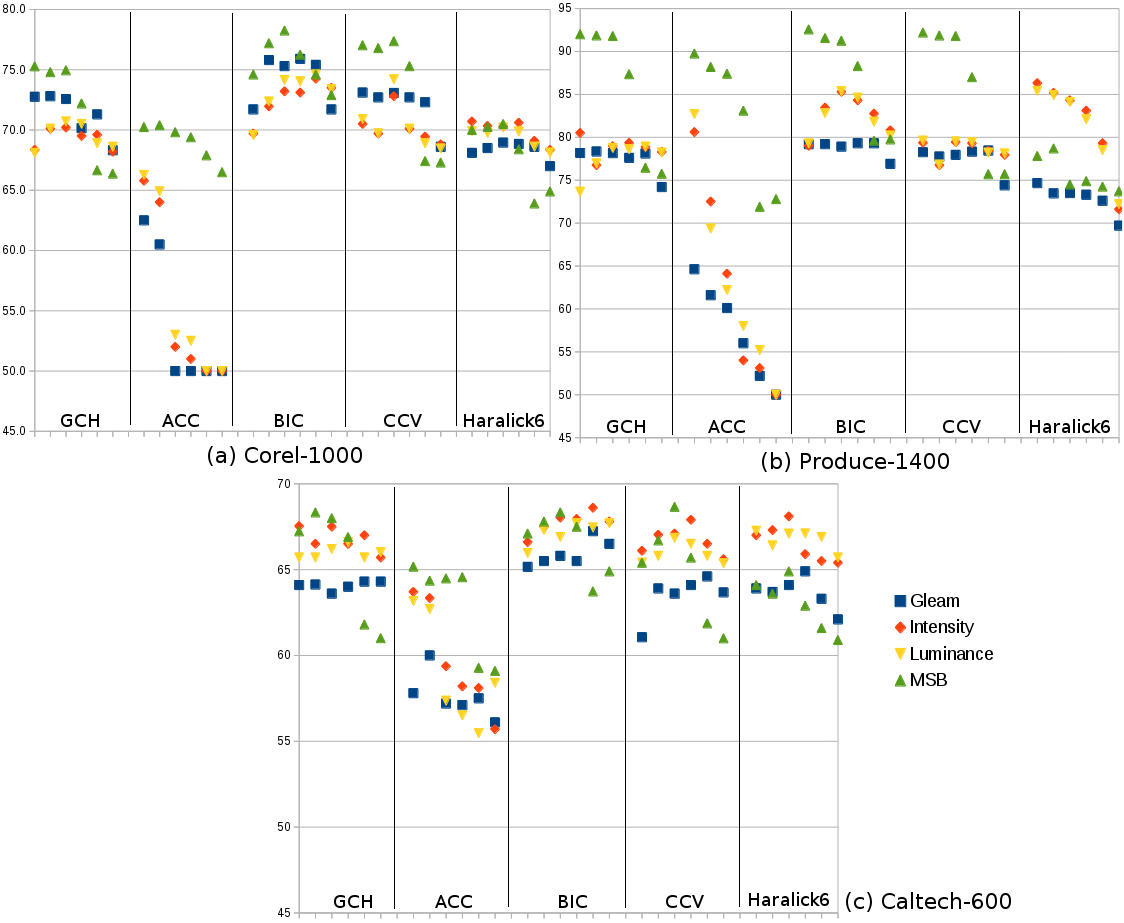
\includegraphics[width=\linewidth]{\detokenize{figuras/quantizacao/fig_results_individual.png}}
  \end{center}
  \caption[Resultados para Corel(a), Produce(b) e Caltech(c), utilizando todos os métodos de quantização. Para cada método de extração de características a acurácia é resultante da sua aplicação utilizando 256, 128, 64, 32, 16 e 8 cores, da esquerda para a direita.]{Resultados para Corel(a), Produce(b) e Caltech(c), com todos os métodos de quantização. Para cada método de extração de características a acurácia é resultante da sua aplicação utilizando 256, 128, 64, 32, 16 e 8 cores, da esquerda para a direita.\textit{Fonte:~\cite{Ponti2016}.}}
  \label{fig:quant:results}
\end{figure}

A partir dessa análise geral, uma análise mais específica foi realizada com a combinação dos métodos BIC e MSB; e Haralick e Luminância. Considerando que a utilização de apenas 16 e 8 cores resultou em uma acurácia muito inferior, o restante dos resultados utilizam 256, 128, 64 e 32 cores.

\meutodo{descrever o teste estatístico e o resultado}

O teste estatístico ANOVA foi realizado para comparar as acurácias dos experimentos da Figura \ref{fig:quant:boxplotBIC} e \ref{fig:quant:boxplotHaralick}. O boxplot para 256, 128, 64 e 32 cores com os métodos BIC e MSB está demonstrado na Figura \ref{fig:quant:boxplotBIC}. De acordo com o teste estatístico representado, utilizar características de cor e níveis de quantização providos pelo método MSB demonstrou resultados melhores do que com 256 cores para as bases Corel (128, 64 e 32 cores) e Caltech (64 cores). O único resultado que piorou significativamente foi para 32 cores da base de imagens \textit{Produce}. Portanto, reduzir converter as imagens de 3 canais de cores para um e reduzir os 256 possíveis valores para apenas 64 provou uma boa escolha de processamento anterior a extração de características. Menores valores podem degradar os resultados em características de textura, como mostrado na Figura \ref{fig:quant:boxplotHaralick}.

\begin{figure}[htbp]
  \begin{center}
    \centering
    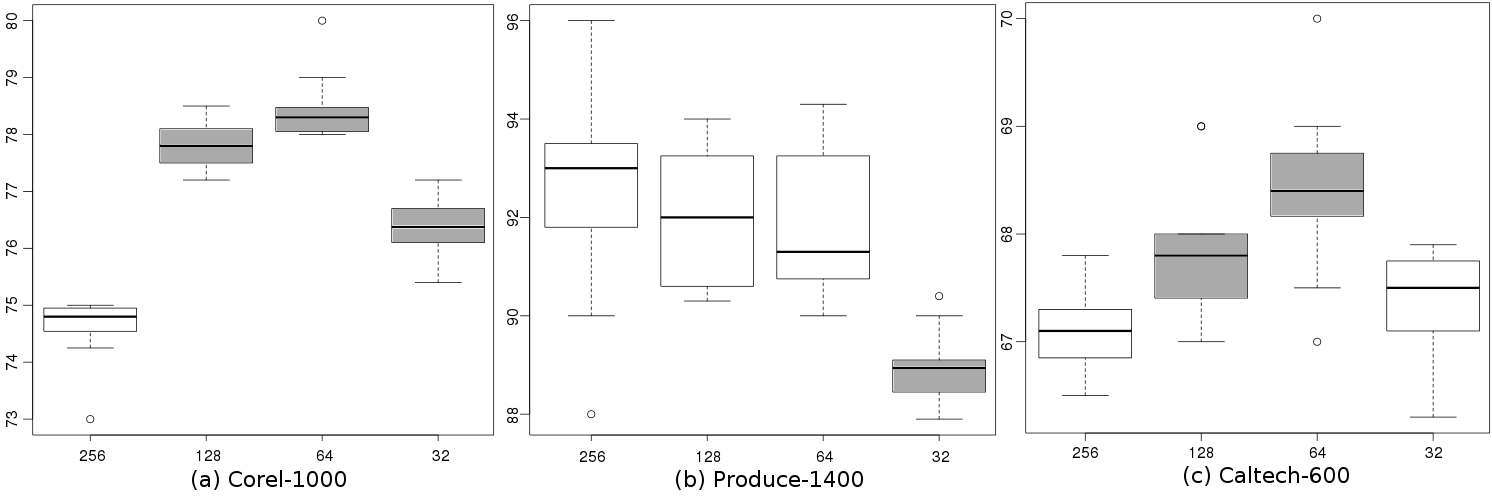
\includegraphics[width=\linewidth]{\detokenize{figuras/quantizacao/fig_results_individual_boxplotBIC.png}}
  \end{center}
  \caption[Resultados de acurácia para o método de quantização MSB considerando 256, 128, 64 e 32 cores com o descritor BIC. Os boxplots em cinza correspondem às significâncias estatísticas com $p \l 0.01$ quando comparado a acurácia de 256 cores.]{Resultados de acurácia para o método de quantização MSB considerando 256, 128, 64 e 32 cores com o descritor BIC. Os boxplots em cinza correspondem às significâncias estatísticas com $p \l 0.01$ quando comparado a acurácia de 256 cores. \textit{Fonte:~\cite{Ponti2016}.}}
  \label{fig:quant:boxplotBIC}
\end{figure}

\begin{figure}[htbp]
  \begin{center}
    \centering
    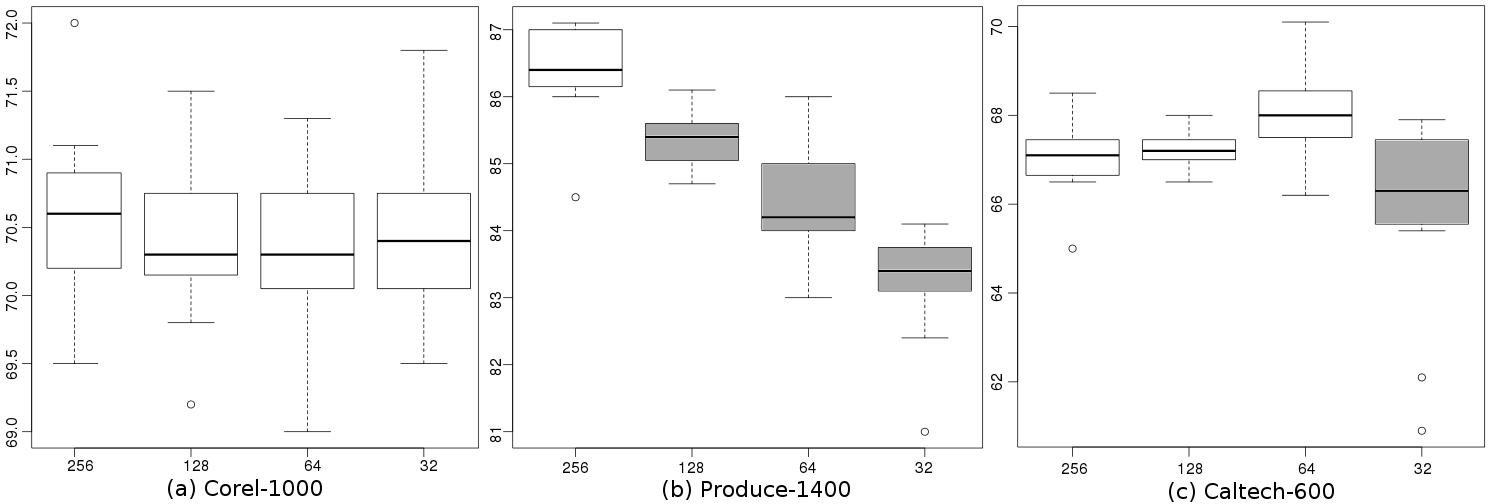
\includegraphics[width=\linewidth]{\detokenize{figuras/quantizacao/fig_results_individual_boxplotHaralick.png}}
  \end{center}
  \caption[Resultados de acurácia para o método de quantização Luminância considerando 256, 128, 64 e 32 cores com o descritor Haralick. Os boxplots em cinza correspondem às significâncias estatísticas com $p \l 0.01$ quando comparado a acurácia de 256 cores.]{Resultados de acurácia para o método de quantização Luminância considerando 256, 128, 64 e 32 cores com o descritor Haralick. Os boxplots em cinza correspondem às significâncias estatísticas com $p \l 0.01$ quando comparado a acurácia de 256 cores. \textit{Fonte:~\cite{Ponti2016}.}}
  \label{fig:quant:boxplotHaralick}
\end{figure}

A redução de dimensionalidade obtida utilizando os métodos de quantização e redução da dimensionalidade com o LPP está ilustrada na Figura \ref{fig:quant:boxplotMSBLPP}. A imagem de entrada foi convertida para escala de cinza com o método MSB em 256 cores. Essa imagem foi dada como entrada para o método de extração de características BIC, que resultou em um vetor dado como entrada para o LPP. Esse último passo teve o objetivo de produzir versões reduzidas desse vetor para 256, 128 e 64 dimensões. As acurácias obtidas foram comparadas com a classificação dos vetores reduzidos apenas pela quantização. O método de quantização obteve valores de acurácia menores à utilização do LPP em três experimentos: de 256 dimensões com a base \textit{Corel} e com 256 e 64 na base \textit{Produce}. Para a base \textit{Caltech} a quantização foi melhor com 256 e 128 dimensões. O restante dos experimentos não apresentaram diferença estatística relevante. Apesar da perda de acurácia em alguns casos, é importante notar que -- se utilizado um número de cores correto -- é possível manter ou até mesmo melhorar as acurácias após a redução da dimensionalidade. Isso pode ser observado na Figura \ref{fig:quant:boxplotMSBLPP} referente à base de dados \textit{Caltech}.

\begin{figure}[htbp]
  \begin{center}
    \centering
    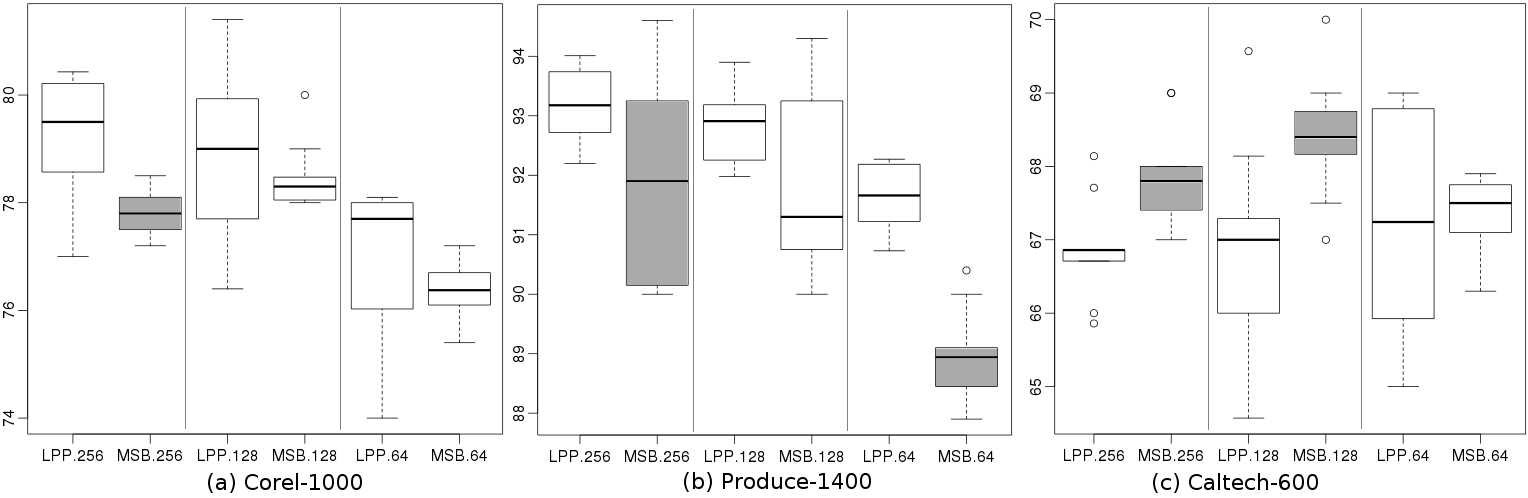
\includegraphics[width=\linewidth]{\detokenize{figuras/quantizacao/fig_results_individual_boxplotMSBLPP.png}}
  \end{center}
  \caption[Resultados de acurácia para os método MSB (quantização), LPP (redução de dimensionalidade) e BIC (extração de características). A comparação do LPP versus MSB foi realizada com a mesma dimensionalidade. Os boxplots em cinza correspondem às significâncias estatísticas com $p \l 0.01$ quando comparado a acurácia de 256 cores.]{Resultados de acurácia para os método MSB (quantização), LPP (redução de dimensionalidade) e BIC (extração de características). A comparação do LPP versus MSB foi realizada com a mesma dimensionalidade. Os boxplots em cinza correspondem às significâncias estatísticas com $p \l 0.01$ quando comparado a acurácia de 256 cores. \textit{Fonte:~\cite{Ponti2016}.}}
  \label{fig:quant:boxplotMSBLPP}
\end{figure}

O número de dimensões de um vetor resultante de apenas um método de extração de características pode ser considerado baixo. Ainda mais que é comum extrair diversos descritores para uma situação, considernado que normalmente não está claro qual método deveria ser utilizado em cada caso. Por conta disso, os próximos experimentos utilizaram a concatenação de tais características. O objetivo destes experimentos é verificar se a concatenação de todos os descritores pode melhorar os resultados de acurácia. Além disso, comparar os resultados com os experimentos anteriores, afim de verificar se a quantização pode ser uma alternativa a redução da dimensionalidade com métodos convencionais (LPP, neste caso). A melhor configuração encontrada, até então, entre tamanho do vetor e acurácia foi utilizando 128 e 64 cores.

Inicialmente, foi testada a configuração de um vetor $D=2310$ com LPP para redução de dimensionalidade com $d$ = 1160, 582, 294 e 150. Ou seja, produzindo vetores com o mesmo tamanho dos obtidos apenas com a quantização como redução da dimensão. O número de características em relação ao número de cores, concatenando todos os vetores resultantes dos métodos de extração de características, é: 256 cores -- 2310 características; 128 cores -- 1160 características; 64 cores -- 582 características; 32 cores --- 294 características; e 16 cores -- 150 características. A Figura \ref{fig:quant:resultsFull} mostra os resultados utilizando LPP. Note que o método de quantização MSB resultou em acurácias melhores que os outros métodos.

\begin{figure}[htbp]
  \begin{center}
    \centering
    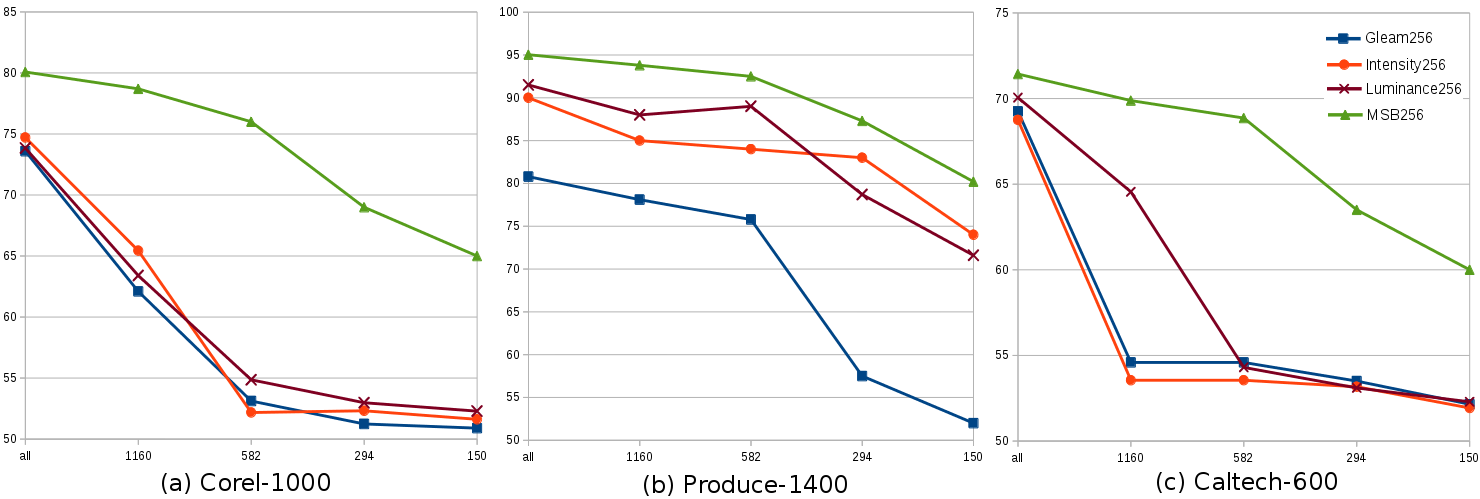
\includegraphics[width=\linewidth]{\detokenize{figuras/quantizacao/fig_results_full.png}}
  \end{center}
  \caption[Comparação da acurácia alcançada com diferentes métodos de quantização: Gleam, Intensidade, Luminância e MSB. Inicialmente com $D=2310$ e então reduzindo com LPP para $d = 1160$, $582$, $294$ e $150$.]{Comparação da acurácia alcançada com diferentes métodos de quantização: Gleam, Intensidade, Luminância e MSB. Inicialmente com $D=2310$ e então reduzindo com LPP para $d = 1160$, $582$, $294$ e $150$. \textit{Fonte:~\cite{Ponti2016}.}}
  \label{fig:quant:resultsFull}
\end{figure}

A utilização da concatenação de todos os vetores melhorou a acurácia em relação ao melhor descritor individual. A Figura \ref{fig:quant:resultsFullBoxplot} apresenta a comparação do espaço original com LPP e MSB para redução da dimensionalidade. O teste estatístico ANOVA foi realizado utilizando $\alpha = 0.01$ como nível de significância. Os resultados que não mudaram significativamente as acurácias foram: MSB com 582 características para a base de dados Corel; e MSB com 1160 nas três bases. O único resultado de piora significative foi para 32 cores com a base Produce. Por conta disso, 64 cores parece ser uma boa escolha de parâmetro de quantização.

\begin{figure}[htbp]
  \begin{center}
    \centering
    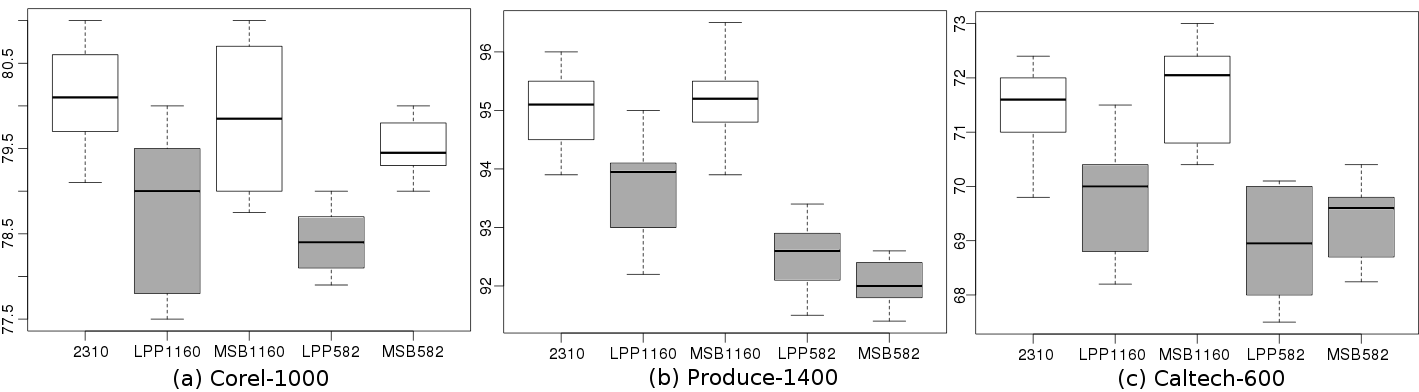
\includegraphics[width=\linewidth]{\detokenize{figuras/quantizacao/fig_results_full_boxplot.png}}
  \end{center}
  \caption[Comparação da acurácia com o uso da projeção LPP e o método MSB para quantização das imagens com o objetivo de redução de dimensionalidade.]{Comparação da acurácia com o uso da projeção LPP e o método MSB para quantização das imagens com o objetivo de redução de dimensionalidade. \textit{Fonte:~\cite{Ponti2016}.}}
  \label{fig:quant:resultsFullBoxplot}
\end{figure}

Os resultados indicam que a quantização pode ser utilizada como redução da dimensão de dados visuais, especialmente utilziando 128 e 64 cores. Como experimento, a Figura \ref{fig:quant:fullLPP} mostra as acurácias resultantes da aplicação do LPP sob o vetor obtido após a quantização com MSB utilizando 256 e 64 cores ($d=2310$ e $d=582$, respectivamente). É interessante notar que as projeções LPP em geral foram melhores com as imagens quantizadas em 64 cores com MSB ao invés da original em 256. A razão para isso deve estar no fato da quantização remover informações confusas: ela simplifica as imagens de forma que as cores restantes possam melhor descrever uma certa classe.

\begin{figure}[htbp]
  \begin{center}
    \centering
    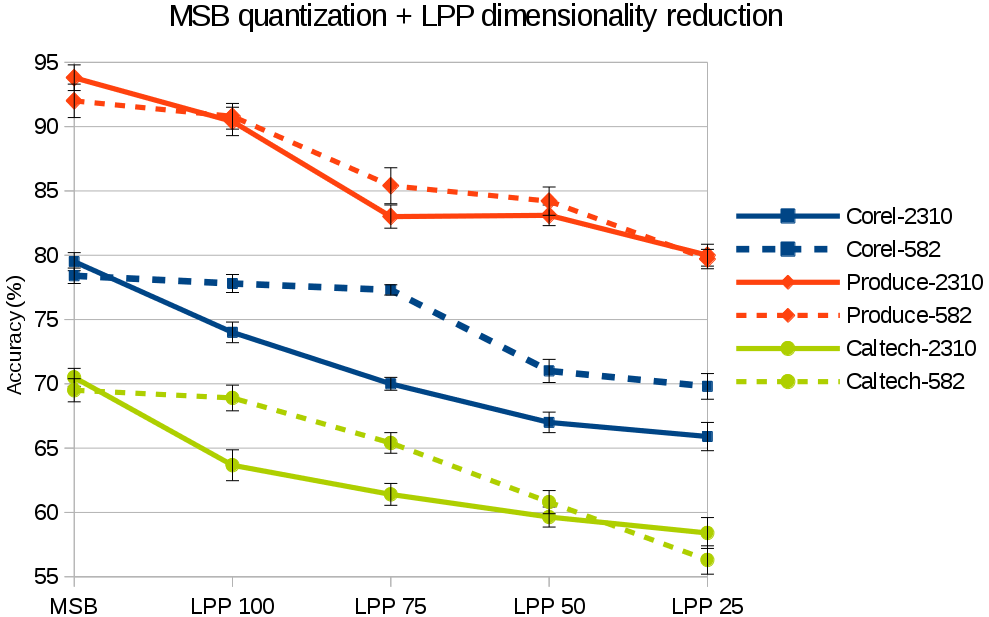
\includegraphics[width=0.6\linewidth]{\detokenize{figuras/quantizacao/fig_results_full_LPP}}
  \end{center}
  \caption[Resultados para a projeção do LPP sobre o espaço de características produzido pelo método de quantização MSB utilizando 256 ($d = 2310$) e 64 cores ($d=582$)]{Resultados para a projeção do LPP sobre o espaço de características produzido pelo método de quantização MSB utilizando 256 ($d = 2310$) e 64 cores ($d=582$)\textit{Fonte:~\cite{Ponti2016}.}}
  \label{fig:quant:fullLPP}
\end{figure}

O vetor concatenado com todos os descritores possui $9C + 6$ dimensões, onde $C$ é o número de cores da imagem de entrada. E o tempo de execução para a extração de todas as características é $f(N) = 42N + 6C^2$, onde $N$ é o número de pixels. Para cada imagem são necessárias $D^2 + kD + d^2$ operações para computar o vetor reduzido com LPP, onde $D$ é o tamanho do vetor original, $d$ o tamanho do vetor de saída e $k$ é o número de vizinhos utilizados no algoritmo.

Ao comparar o uso da quantização com a utilização de métodos mais complexos para redução da dimensionalidade, esse procedimento permite uma redução significante, enquanto normalmente preserva ou melhora a acurácia do sistema. Independente da utilização de um método de seleção de características, ao escolher um método de quantização apropriado e seus parâmetros é possível reduzir a dimensionalidade e acelerar computacionalmente as etapas que precedem o reconhecimento de imagens. Considere o seguinte exemplo: 100 imagens com 256 cores demandam 231.6 milhões de instruções para extrair as características e reduzir o vetor utilizando o método LPP (com $k = 10$ e $d = 50$). Se ao invés disso, fossem utilizadas 64 cores, esse número cairia para 58.7 milhões, o que corresponde a uma redução de 74,6\%.

%%%%%%%%%%%%%%%%%%%%%%%%%%%%%%%%%%%%%%%%%%%%%%%%%%%%%%%%%%%%%%%%%%%%%%%%%%%%%%%%

\newpage
\section{Geração de Imagens Artificiais}

Esta seção descreve os resultados encontrados ao rebalancear as classes de imagens utilizando os processamentos descritos no capítulo anterior aplicados nas imagens originais. Na Figura \ref{fig:fluxo} é possível observar o fluxo de operações realizadas para analisar o impacto da geração de imagens no rebalanceamento de classes. O mesmo protocolo de conversão para escala de cinza, extração de características e classificação foi seguido para três experimentos: base desbalanceada; base rebalanceada com interpolação dos vetores de características (método SMOTE); e base rebalanceada com a geração artificial de imagens.

\begin{figure}[thpb]
\centering
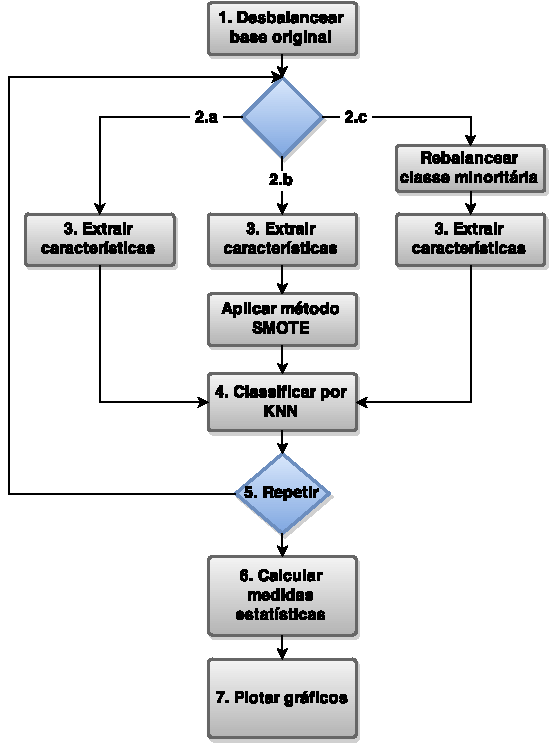
\includegraphics[scale=1]{\detokenize{figuras/flow_main.pdf}}
\caption[Fluxo de operações para obtenção dos resultados do rebalanceamento de classes]{Fluxo de operações para obtenção dos resultados do rebalanceamento de classes. \textit{Fonte:~Elaborado pela autora.}}
\label{fig:fluxo}
\end{figure}

Procurando uma certa estabilidade dos resultados obtidos com a geração das imagens artificiais, foi identificada a necessidade de controlar a remoção de imagens da base no momento da criação da base desbalanceada. Assim, os resultados foram obtidos a partir de uma forma de validação K-fold com o objetivo de prover mais robustez ao sistema. A Figura \ref{fig:folds} ilustra como isso foi realizado. Primeiramente as imagens foram divididas de forma aleatória em $k=5$ folds para cada classe. Depois, as duas classes compõe 40 configurações, consistindo de um fold para teste e os outros para treino na classe que ficará balanceada e um de teste e um de treino para a que os métodos de processamento irão rebalancear.

\begin{figure}[thpb]
\centering
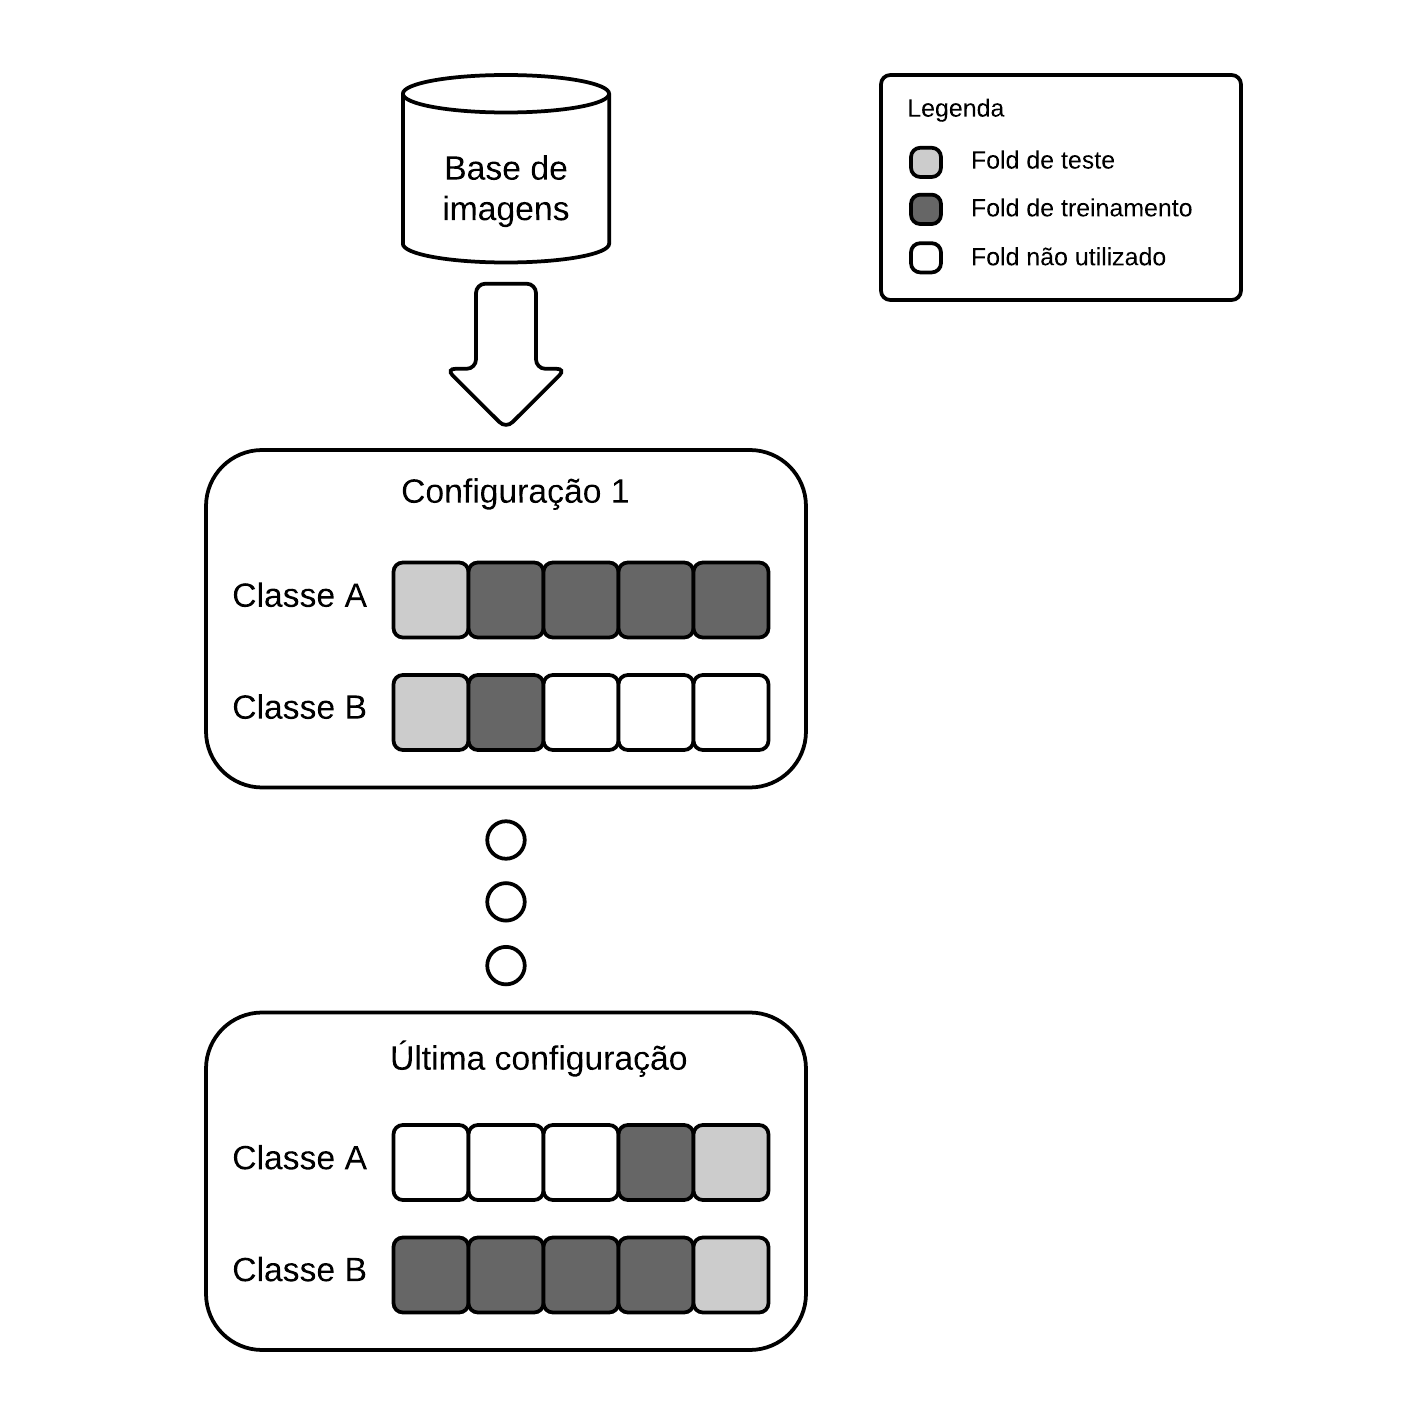
\includegraphics[scale=0.25]{\detokenize{figuras/folds_chart.png}}
\caption[]{\textit{Fonte:~Elaborado pela autora.}}
\label{fig:folds}
\end{figure}

A seguir, para cada base de imagens utilizada, são descritos: a base em si; o protocolo e parâmetros adotados; e por fim os resultados obtidos a partir de seu uso são mostrados e discutidos.

%%%%%%%%%%%%%%%%%%%%%%%%%%%%%%%%%%%%%%%%%%%%%%%%%%%%%%%%%%%%%%%%%%%%%%%%%%%%%%%%
\subsection{Experimento 1: duas classes bem discriminadas}

\begin{itemize}
%%%%%%%%%%%%%%%%%%%%%%%%%%%%%%%%%%%%%%%%%%%%%%%%%%%%%%%%%%%%%%%%%%%%%%%%%%%%%%%%
\item[] \textbf{Base de Imagens}

Neste experimento foram utilizadas duas classes da base Corel de cavalos e elefantes. Elas estão exemplificadas na Figura \ref{fig:exp1:base}. A principal característica dessas imagens é a grande diferença das cores das imagens, apesar de haverem casos de confusão.

\begin{figure}[htbp]
  \begin{center}
    \begin{subfigure}{.4\linewidth}
      \centering
      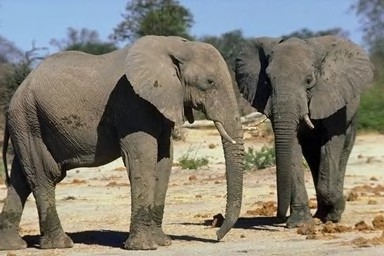
\includegraphics[width=\linewidth]{\detokenize{figuras/corel_original4.jpg}}
    \end{subfigure}
    \begin{subfigure}{.4\linewidth}
      \centering
      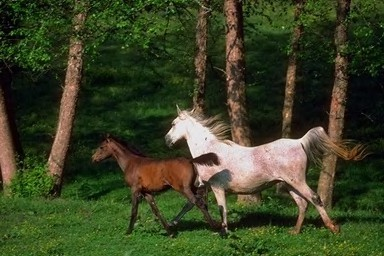
\includegraphics[width=\linewidth]{\detokenize{figuras/cavalo-original2.png}}
    \end{subfigure}
  \end{center}
  \caption[]{Classes cavalo e elefante utilizadas neste experimento. São duas classes com 100 imagens cada, originalmente da base de imagens Corel. \textit{Fonte:~Elaborado pela autora.}}
  \label{fig:exp1:base}
\end{figure}

%%%%%%%%%%%%%%%%%%%%%%%%%%%%%%%%%%%%%%%%%%%%%%%%%%%%%%%%%%%%%%%%%%%%%%%%%%%%%%%%
\item[] \textbf{Protocolo}

\begin{enumerate}
\item \textbf{Imagens originais}: classes \emph{elefante} e \emph{cavalo} da Corel;
\item \textbf{Desbalanceamento}: para a visualização cada classe foi dividida em 50\% para treino e 50\% para teste e após a classe \emph{cavalo} sofreu remoção de 50\% do conjunto de treino. Já para a análise estatística, todas as 40 configurações de folds com $k=5$ foram realizadas;
\item \textbf{Método para geração artificial}: para a visualização do espaço de características consistiu na mistura de duas imagens originais, exemplificado na Figura~\ref{fig:mistura}. Para a análise do boxplot de f1-scores, todas as gerações foram testadas;
\item \textbf{Quantização}: Intensidade;
\item \textbf{Extração de características}: classificação de pixels de borda e interior (BIC);
\item \textbf{Classificação}: classificador supervisionado KNN com $K=1$ (para mais detalhes ver Seção~\ref{sec:knn});
\item \textbf{Projeção multidimensional}: projetados os dois componentes principais encontrados ao aplicar PCA nos vetores de características para redução de dimensionalidade (Seção~\ref{sec:pca}).
% A implementação desenvolvida para esta projeção pode ser encontrada em \url{https://github.com/GabiThume/msc-src/blob/master/visualization/plot.py}. Vale destacar que uma animação da adição de cada novo exemplo foi realizada para fim de visualizar o melhor subespaço gerado.
\end{enumerate}

\begin{figure}[htbp]
  \begin{center}
    \begin{subfigure}{.3\linewidth}
      \centering
      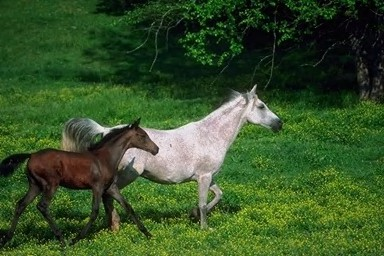
\includegraphics[width=\linewidth]{\detokenize{figuras/cavalo-original.png}}
    \caption{Original}
    \end{subfigure}
    \begin{subfigure}{.3\linewidth}
      \centering
      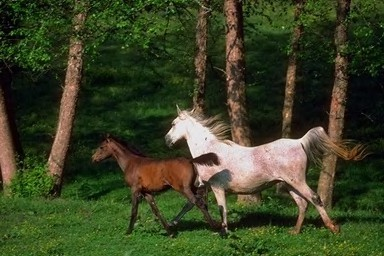
\includegraphics[width=\linewidth]{\detokenize{figuras/cavalo-original2.png}}
    \caption{Original}
    \end{subfigure}
    \begin{subfigure}{.3\linewidth}
      \centering
      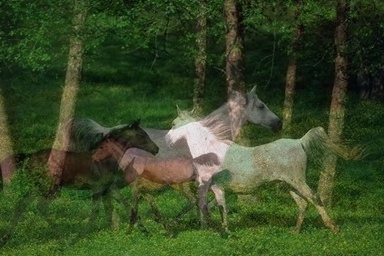
\includegraphics[width=\linewidth]{\detokenize{figuras/cavalo-blend.png}}
    \caption{Mistura}
  \end{subfigure}
  \end{center}
  \caption{Geração artificial de imagens com o método de mistura.}
  \label{fig:mistura}
\end{figure}

%%%%%%%%%%%%%%%%%%%%%%%%%%%%%%%%%%%%%%%%%%%%%%%%%%%%%%%%%%%%%%%%%%%%%%%%%%%%%%%%
\item[] \textbf{Resultados e Discussão}


%%%%%%%%%%%%%%%%%%%%%%%%%%%%%%%%%%%%%%%%%%%%%%%%%%%%%%%%%%%%%%%%%%%%%%%%%%%%%%%%
\item[] \textbf{Visualização}

As classes \emph{elefante} e \emph{cavalo} possuem 100 imagens cada. O primeiro passo é remover imagens de uma das classes, tornando a base desbalanceada. Como o foco é na visualização do espaço de características, é relevante ter o modelo do espaço ideal das classes balanceadas, por isso esse experimento em específico não trata de uma base naturalmente desbalanceada. Na Figura~\ref{fig:desbalanceado} está ilustrada a remoção de 50\% das imagens de treino da classe \emph{cavalo}, originalmente balanceada. Essa e as próximas projeções desta seção foram obtidas com a técnica para redução de dimensionalidade PCA, descrita na Seção~\ref{sec:pca} e são referentes aos dois componentes principais com maiores autovalores.

\begin{figure}[htbp]
  \begin{center}
    \begin{subfigure}{.49\linewidth}
      \centering
      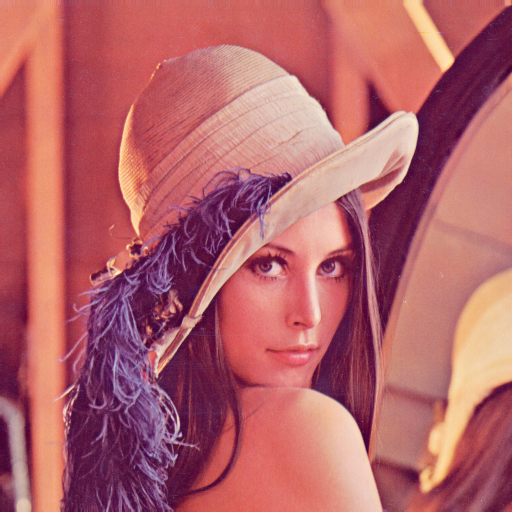
\includegraphics[width=\linewidth]{\detokenize{figuras/visualizacao/original.png}}
    \end{subfigure}
    \begin{subfigure}{.49\linewidth}
      \centering
      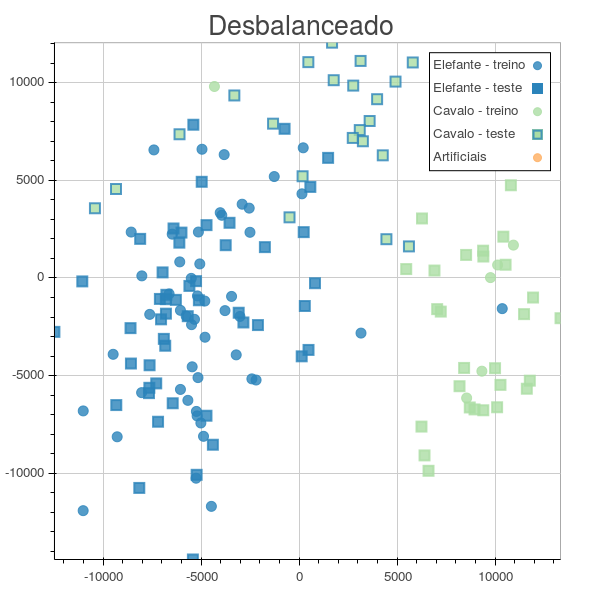
\includegraphics[width=\linewidth]{\detokenize{figuras/visualizacao/desbalanceado-fixed.png}}
    \end{subfigure}
  \end{center}
  \caption{Remoção de 50\% das imagens de treino da classe \emph{cavalo}.}
  \label{fig:desbalanceado}
\end{figure}

A classificação dos três experimentos utilizando KNN reportou que o \textit{f-score} da geração artificial de imagens utilizando o método de mistura teve um ganho de mais de 10\% em relação ao rebalanceamento no espaço de características com o SMOTE. Para confirmar que a geração aqui proposta inseriu mais informação na classe minoritária do que apenas povoar os espaços entre os exemplos (i.e.\ SMOTE), a classe rebalanceada utilizando ambos métodos está demonstrada na Figura~\ref{fig:compara_vis_treino_fixed}. Em laranja estão representados os novos exemplos de treinamento, projetados no plano da base original balanceada.

\begin{figure}[htbp]
  \begin{center}
    \begin{subfigure}{.49\linewidth}
      \centering
      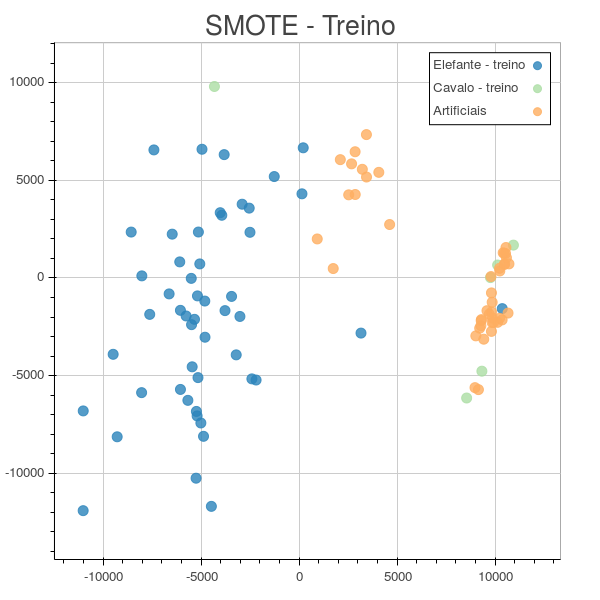
\includegraphics[width=\linewidth]{\detokenize{figuras/visualizacao/smote-treino-fixed.png}}
    \end{subfigure}
    \begin{subfigure}{.49\linewidth}
      \centering
      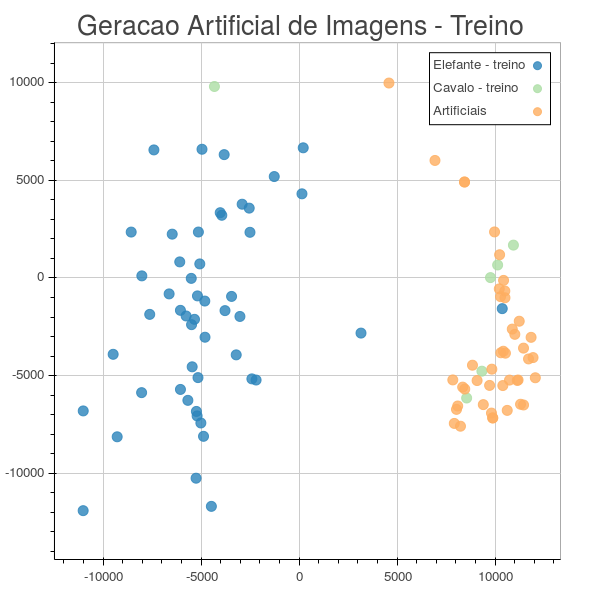
\includegraphics[width=\linewidth]{\detokenize{figuras/visualizacao/geracao-treino-fixed.png}}
    \end{subfigure}
  \end{center}
  \caption{Comparação dos exemplos de treinamento da geração com SMOTE e no campo visual. Em laranja estão representados os novos exemplos, projetados no plano da base original balanceada.}
  \label{fig:compara_vis_treino_fixed}
\end{figure}

Após o treinamento realizado com as novas imagens e exemplos, o conjunto de teste foi fornecido ao classificador 1-NN e o resultado das predições está ilustrado na Figura~\ref{fig:compara_vis_teste}. A cor no interior dos marcadores quadrados representa a classe real dos exemplos e a borda representa a classe predita pelo classificador. Nota-se que a melhoria na classificação com a geração de imagens fica visível e corresponde ao aumento do \textit{f-score}.

\begin{figure}[htbp]
  \begin{center}
    \begin{subfigure}{.49\linewidth}
      \centering
      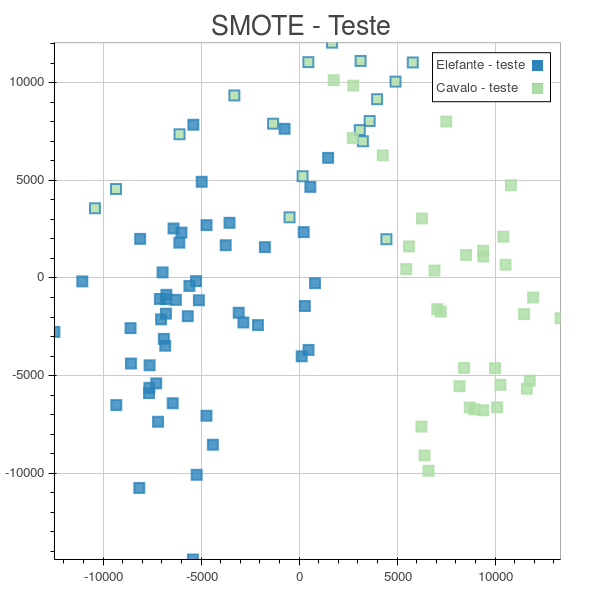
\includegraphics[width=\linewidth]{\detokenize{figuras/visualizacao/smote-teste-fixed.png}}
    \end{subfigure}
    \begin{subfigure}{.49\linewidth}
      \centering
      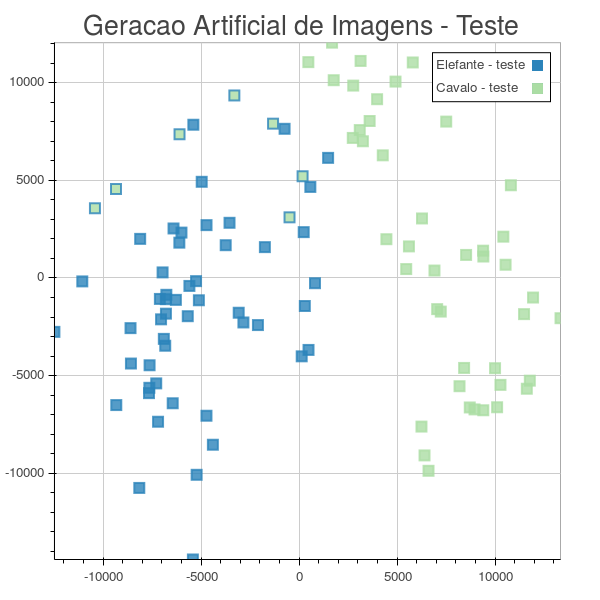
\includegraphics[width=\linewidth]{\detokenize{figuras/visualizacao/geracao-teste-fixed.png}}
    \end{subfigure}
  \end{center}
  \caption{Resultado do teste da classificação com 1-NN após o treinamento realizado com as bases rebalanceadas. A cor no interior dos marcadores quadrados representa a classe real dos exemplos e a borda representa a classe predita pelo classificador.}
  \label{fig:compara_vis_teste}
\end{figure}

De uma forma geral, pode-se dizer que a geração de imagens melhorou a definição da classe minoritária e foi o método que mais se assemelhou à distribuição dos dados originais. Além disso, um dos problemas do SMOTE pode ser verificado nessas projeções: ao realizar a interpolação dos vetores de características originais, pode-se criar exemplos em regiões do espaço que fazem parte da outra classe. Ficou claro também que o método SMOTE não possui capacidade de extrapolar a sua região, como pode ser observado no grupo de exemplos gerados à direita do espaço. O SMOTE gerou novos elementos em linha reta, enquanto a geração de imagens proporcionou uma abrangência maior em volta desse espaço, com maior dispersão.

É válido também visualizar a região de decisão, observando suas modificações frente aos métodos. Pode ser observado que em ambas técnicas a região da classe minoritária apresenta-se melhor representada. Além disso, é possível verificar que o SMOTE ocasionou uma certa ``invasão'' do espaço de características da classe majoritária.

\begin{figure}[htbp]
  \begin{center}
    \begin{subfigure}{.3\linewidth}
      \centering
      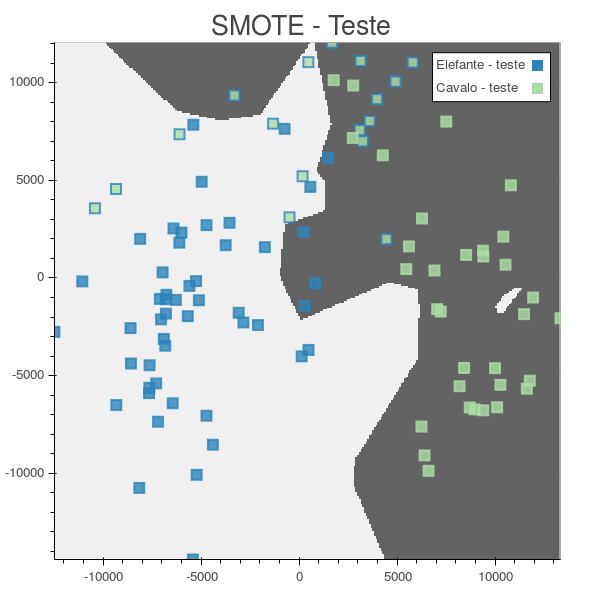
\includegraphics[width=\linewidth]{\detokenize{figuras/visualizacao/smote-teste-region.png}}
    \end{subfigure}
    \begin{subfigure}{.3\linewidth}
      \centering
      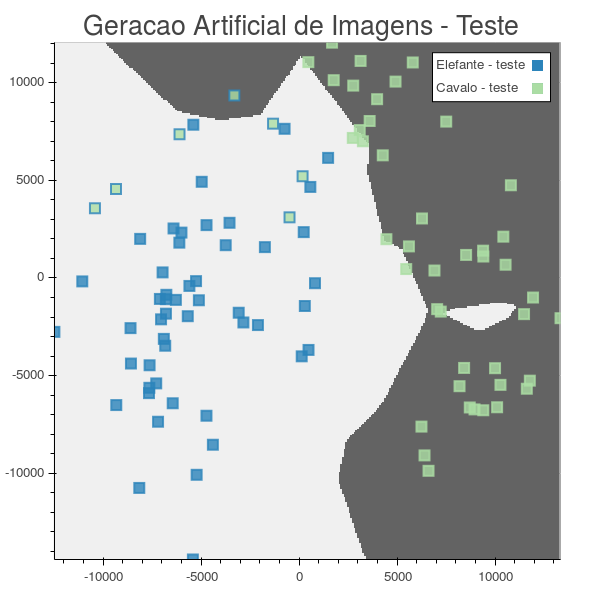
\includegraphics[width=\linewidth]{\detokenize{figuras/visualizacao/geracao-teste-region.png}}
    \end{subfigure}
    \begin{subfigure}{.3\linewidth}
      \centering
      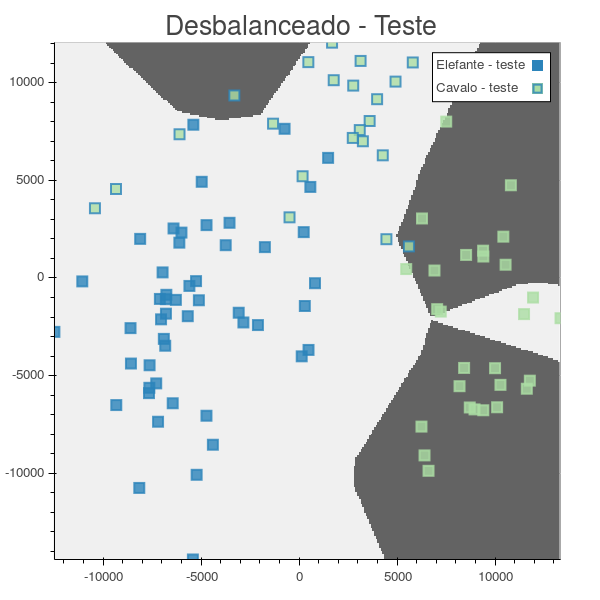
\includegraphics[width=\linewidth]{\detokenize{figuras/visualizacao/desbalanceado-teste-region.png}}
    \end{subfigure}
  \end{center}
  \caption{Região de decisão com K-NN (K = 1)}
  \label{fig:region}
\end{figure}

Nas figuras anteriores os exemplos foram projetados no plano criado pelas suas componentes principais com maior autovalores da base original balanceada. Se após a geração de novos exemplos essas componentes forem recalculadas (Figura \ref{fig:compara_vis_treino}), pode-se notar que a geração de imagens artificiais proporciona a criação de um subespaço que melhor discretiza as classes, quando comparado com SMOTE ou com a base desbalanceada.

\begin{figure}[htbp]
  \begin{center}
    \begin{subfigure}{.3\linewidth}
      \centering
      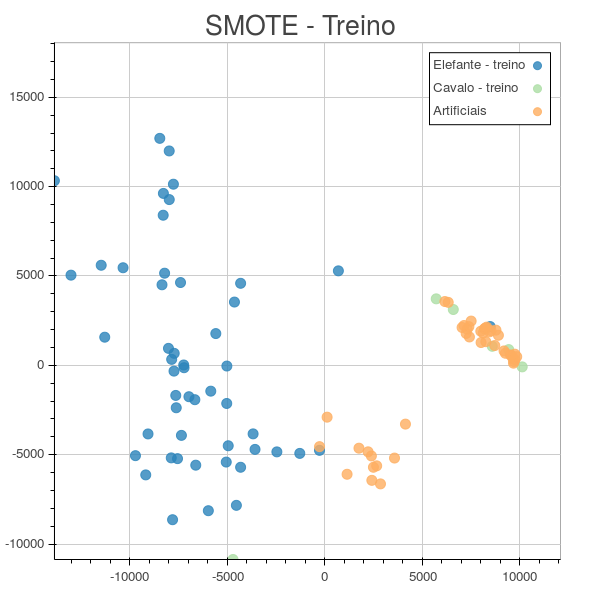
\includegraphics[width=\linewidth]{\detokenize{figuras/visualizacao/smote-treino.png}}
    \end{subfigure}
    \begin{subfigure}{.3\linewidth}
      \centering
      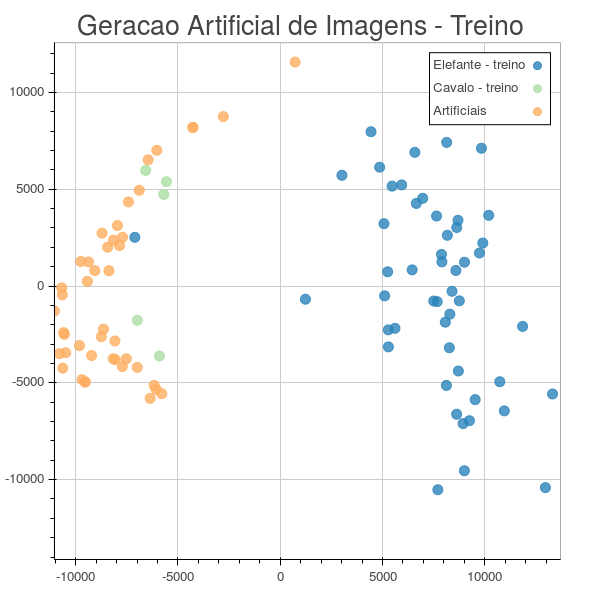
\includegraphics[width=\linewidth]{\detokenize{figuras/visualizacao/geracao-treino.png}}
    \end{subfigure}
    \begin{subfigure}{.3\linewidth}
      \centering
      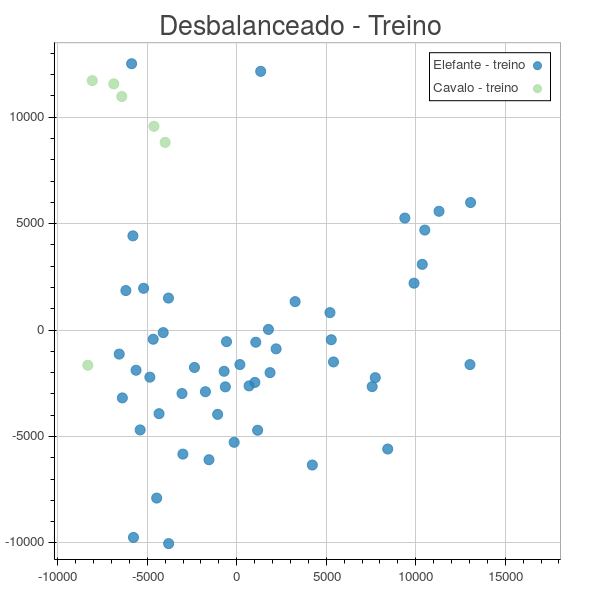
\includegraphics[width=\linewidth]{\detokenize{figuras/visualizacao/desbalanceado-treino.png}}
    \end{subfigure}
  \end{center}
  \caption{Melhores subespaços encontrados após a geração de novos exemplos para o SMOTE e para a geração artificial de imagens, e após a remoção de imagens para a projeção dos dados desbalanceados.}
  \label{fig:compara_vis_treino}
\end{figure}

Como relatado no início dessa seção, o extrator de características utilizado foi o BIC. Fundamentalmente ele captura informações de intensidade de cor das imagens. Na Figura~\ref{fig:vis_images} as próprias imagens foram utilizadas como marcadores na projeção do melhor subespaço após a geração artificial com o método de mistura. É nítido o impacto da etapa de extração de características na separação das classes e também no método de geração de imagens antes dessa extração.

\begin{figure}[htbp]
  \begin{center}
      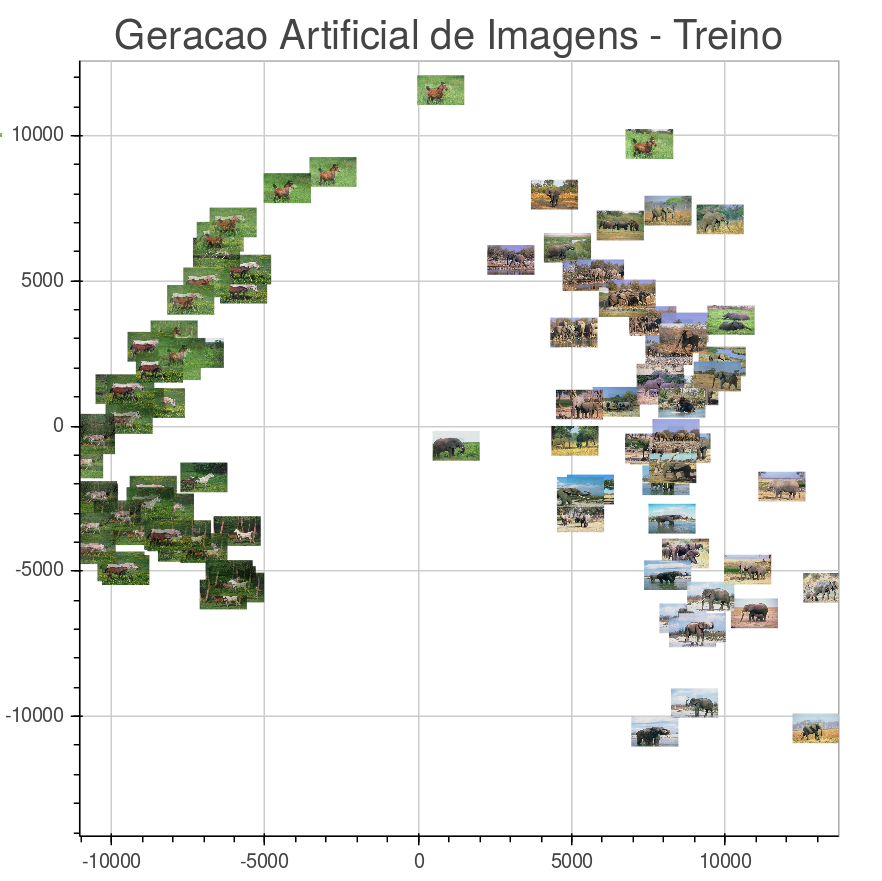
\includegraphics[width=.6\linewidth]{\detokenize{figuras/visualizacao/vis-images.png}}
  \end{center}
  \caption{Visualização do impacto do descritor de características.}
  \label{fig:vis_images}
\end{figure}

\end{itemize}

%%%%%%%%%%%%%%%%%%%%%%%%%%%%%%%%%%%%%%%%%%%%%%%%%%%%%%%%%%%%%%%%%%%%%%%%%%%%%%%%
\subsection{Experimento 2: duas classes bem sobrepostas}

\begin{itemize}
%-------------------------------------------------------------------------------
\item[] \textbf{Base de Imagens}

% \begin{figure}[htbp]
%   \begin{center}
%     \begin{subfigure}{.49\linewidth}
%       \centering
%       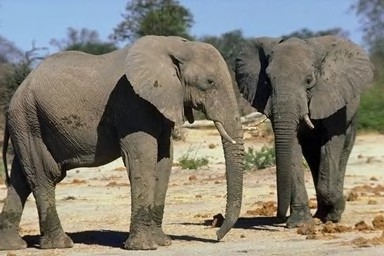
\includegraphics[width=\linewidth]{\detokenize{figuras/corel_original4.jpg}}
%     \end{subfigure}
%     \begin{subfigure}{.49\linewidth}
%       \centering
%       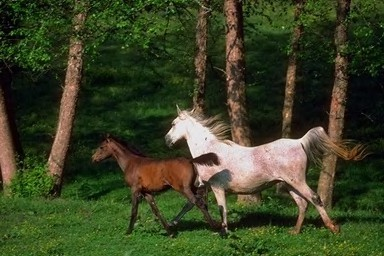
\includegraphics[width=\linewidth]{\detokenize{figuras/cavalo-original2.png}}
%     \end{subfigure}
%   \end{center}
%   \caption{Remoção de 50\% das imagens de treino da classe Cavalo.}
%   \label{fig:exp1:base}
% \end{figure}

%-------------------------------------------------------------------------------
\item[] \textbf{Protocolo}

O seguinte protocolo foi seguido para a obtenção dos resultados:

\begin{enumerate}
\item \textbf{Classes de imagens originais}:
\item \textbf{Desbalanceamento}:
\item \textbf{Método para geração artificial}:
\item \textbf{Quantização}:
\item \textbf{Extração de características}:
\item \textbf{Classificação}:
\end{enumerate}
%-------------------------------------------------------------------------------
\item[] \textbf{Resultados e Discussão}

\end{itemize}

%%%%%%%%%%%%%%%%%%%%%%%%%%%%%%%%%%%%%%%%%%%%%%%%%%%%%%%%%%%%%%%%%%%%%%%%%%%%%%%%
\subsection{Experimento 3: multiclasses}

\begin{itemize}
%-------------------------------------------------------------------------------
\item[] \textbf{Base de Imagens}

% \begin{figure}[htbp]
%   \begin{center}
%     \begin{subfigure}{.49\linewidth}
%       \centering
%       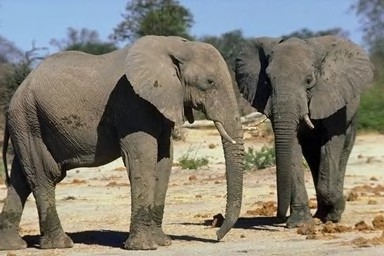
\includegraphics[width=\linewidth]{\detokenize{figuras/corel_original4.jpg}}
%     \end{subfigure}
%     \begin{subfigure}{.49\linewidth}
%       \centering
%       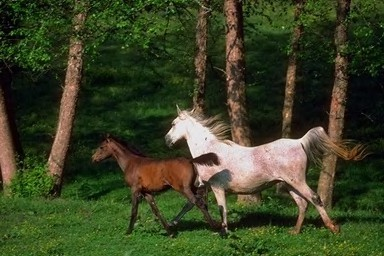
\includegraphics[width=\linewidth]{\detokenize{figuras/cavalo-original2.png}}
%     \end{subfigure}
%   \end{center}
%   \caption{Remoção de 50\% das imagens de treino da classe Cavalo.}
%   \label{fig:exp1:base}
% \end{figure}

%-------------------------------------------------------------------------------
\item[] \textbf{Protocolo}

O seguinte protocolo foi seguido para a obtenção dos resultados:

\begin{enumerate}
\item \textbf{Classes de imagens originais}:
\item \textbf{Desbalanceamento}:
\item \textbf{Método para geração artificial}:
\item \textbf{Quantização}:
\item \textbf{Extração de características}:
\item \textbf{Classificação}:
\end{enumerate}
%-------------------------------------------------------------------------------
\item[] \textbf{Resultados e Discussão}

\end{itemize}

%%%%%%%%%%%%%%%%%%%%%%%%%%%%%%%%%%%%%%%%%%%%%%%%%%%%%%%%%%%%%%%%%%%%%%%%%%%%%%%%
\subsection{Experimento 4: classes naturalmente desbalanceadas}

\begin{itemize}
%-------------------------------------------------------------------------------
\item[] \textbf{Base de Imagens}

% \begin{figure}[htbp]
%   \begin{center}
%     \begin{subfigure}{.49\linewidth}
%       \centering
%       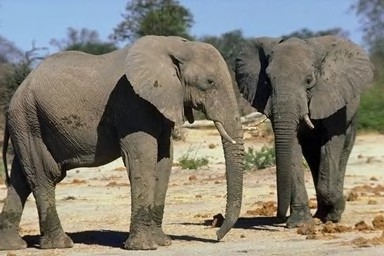
\includegraphics[width=\linewidth]{\detokenize{figuras/corel_original4.jpg}}
%     \end{subfigure}
%     \begin{subfigure}{.49\linewidth}
%       \centering
%       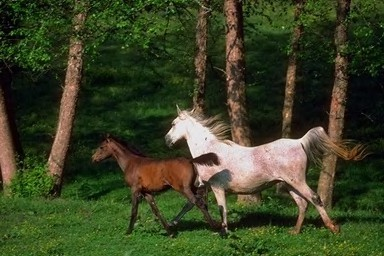
\includegraphics[width=\linewidth]{\detokenize{figuras/cavalo-original2.png}}
%     \end{subfigure}
%   \end{center}
%   \caption{Remoção de 50\% das imagens de treino da classe Cavalo.}
%   \label{fig:exp1:base}
% \end{figure}

%-------------------------------------------------------------------------------
\item[] \textbf{Protocolo}

O seguinte protocolo foi seguido para a obtenção dos resultados:

\begin{enumerate}
\item \textbf{Classes de imagens originais}:
\item \textbf{Desbalanceamento}:
\item \textbf{Método para geração artificial}:
\item \textbf{Quantização}:
\item \textbf{Extração de características}:
\item \textbf{Classificação}:
\end{enumerate}
%-------------------------------------------------------------------------------
\item[] \textbf{Resultados e Discussão}

\end{itemize}


%%%%%%%%%%%%%%%%%%%%%%%%%%%%%%%%%%%%%%%%%%%%%%%%%%%%%%%%%%%%%%%%%%%%%%%%%%%%%%%%
% \begin{figure}[htbp]
%   \begin{center}
%     \begin{subfigure}{.49\linewidth}
%       \centering
%       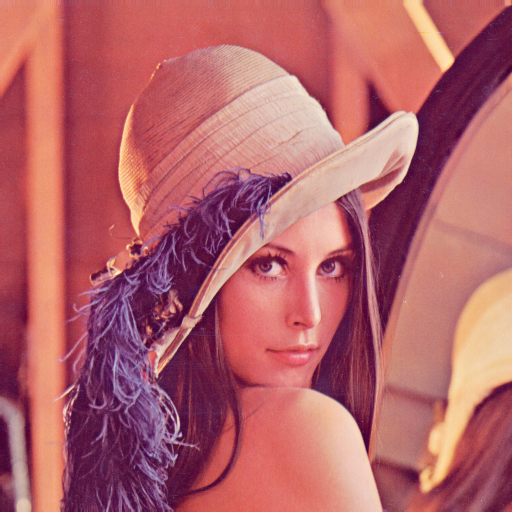
\includegraphics[width=\linewidth]{\detokenize{figuras/visualizacao/original.png}}
%     \end{subfigure}
%     \begin{subfigure}{.49\linewidth}
%       \centering
%       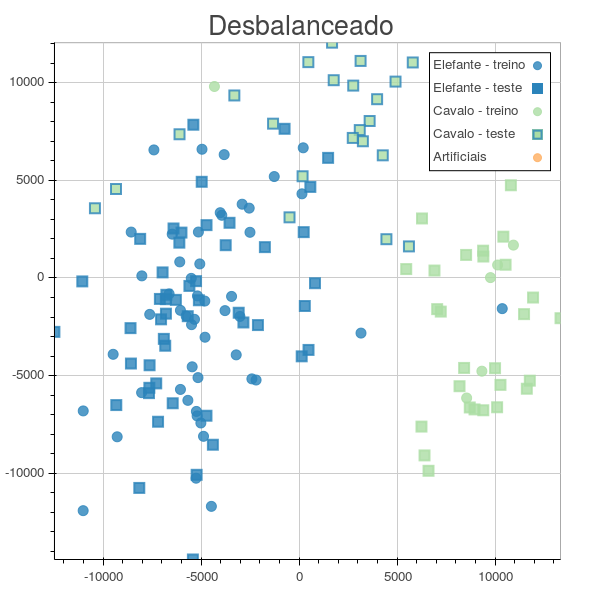
\includegraphics[width=\linewidth]{\detokenize{figuras/visualizacao/desbalanceado-fixed.png}}
%     \end{subfigure}
%   \end{center}
%   \caption{Remoção de 50\% das imagens de treino da classe Cavalo.}
%   \label{fig:desbalanceado}
% \end{figure}

%-------------------------------------------------------------------------------

%  Os resultados foram obtidos utilizando a base de imagens COREL-1000\footnote{Disponível em http://wang.ist.psu.edu/docs/related/}, composta por fotografias que representam classes variadas: tribos africanas, praia, construções, ônibus, dinossauros, elefantes, flores, cavalos, montanhas e tipos de comidas. São 10 classes balanceadas com 100 imagens cada. Para fins de exemplificação, são apresentadas amostras das imagens que representam essas classes na Figura \ref{fig:corel}.
%
%  \begin{figure}[hbpt]
%  \begin{center}
%    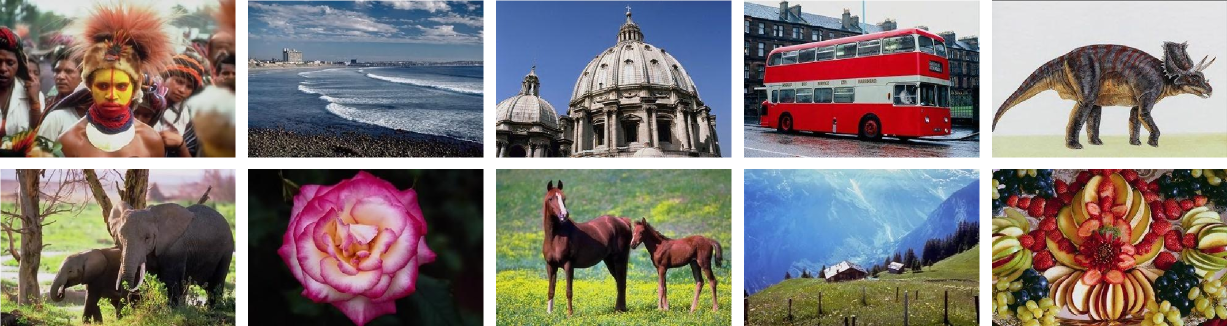
\includegraphics[width=1\linewidth]{\detokenize {figuras/exemplos_corel.png}}
%  \end{center}
%   \caption[Base de imagens COREL-1000.]{Base de imagens COREL-1000 utilizada. Estão representadas as 10 classes da base. \textit{Fonte: Elaborado pela autora.}}
%  \label{fig:corel}
% \end{figure}

% \section{Considerações iniciais}
%
% Este capítulo apresenta os resultados preliminares obtidos. Primeiramente, é apresentada a descrição do experimento realizado, ressaltando os métodos de extração de características, quantização e classificação utilizados. Além disso, o fluxo de operações para a realização do experimento é descrito. Em seguida, os resultados são propriamente ilustrados, ao indicar que a geração de imagens artificiais é promissora para o cenário de bases desbalanceadas. Por fim, as atividades futuras são destacadas.
%
% %--------------------------------------------------------------------------------
% \section{Descrição do experimento}
%
% Algumas pesquisas sobre os efeitos da sobreamostragem e geração de exemplos artificiais em dados de aprendizado de máquina já foram realizadas~\cite{Kuncheva2004,Chawla2002}. O método mais divulgado na literatura é conhecido como SMOTE (\textit{Synthetic Minority Over-sampling Technique}). Este método propõe a geração de exemplos artificiais a partir dos vetores de características originais das classes minoritárias. Não há registro conhecido de um estudo dessas técnicas em dados de informação visual para o rebalanceamento de classes.
%
% % \enlargethispage{-\baselineskip}
%
% Assim, foi proposta a geração de novas imagens a partir de operações como adição de ruído, borramento, mistura e combinação das imagens originais. Tais operações estão exemplificadas na Figura~\ref{fig:ArtificialImages}, utilizando a classe ``praia'' da base de imagens naturais COREL-1000. A partir das imagens originais --- primeira linha da figura --- são geradas imagens artificiais por meio das operações citadas, resultando nas imagens da segunda linha da figura.
%
% \vspace{25pt}
%
% \renewcommand{\tabcolsep}{0.04cm}
% \begin{figure}[!h]
%  \begin{center}
%  \begin{tabular}{ccccc}
%    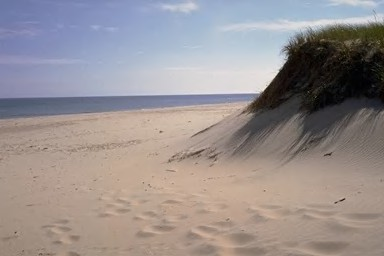
\includegraphics[width=0.245\linewidth]{\detokenize {figuras/original-1.jpg}}&
%    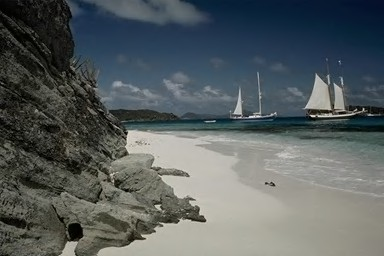
\includegraphics[width=0.245\linewidth]{\detokenize {figuras/original-2.jpg}}&
%    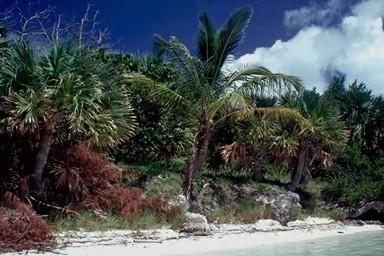
\includegraphics[width=0.245\linewidth]{\detokenize {figuras/original-3.jpg}}&
%    % 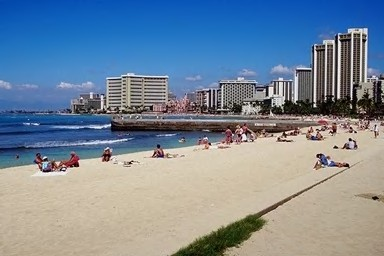
\includegraphics[width=0.19\linewidth]{\detokenize {figuras/original-4.jpg}}&
%    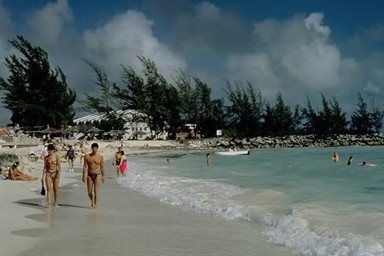
\includegraphics[width=0.245\linewidth]{\detokenize {figuras/original-5.jpg}}\\
%    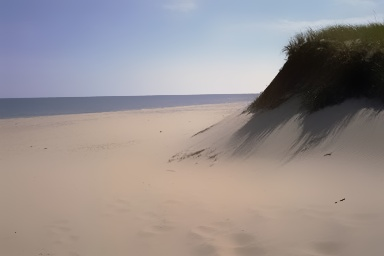
\includegraphics[width=0.245\linewidth]{\detokenize {figuras/gerada-1_blur.jpg}}&
%    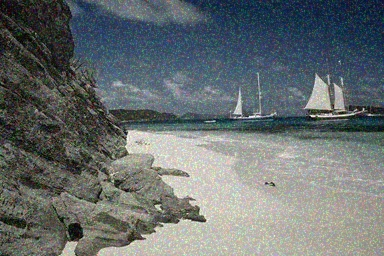
\includegraphics[width=0.245\linewidth]{\detokenize {figuras/gerada-2_ruido.jpg}}&
%    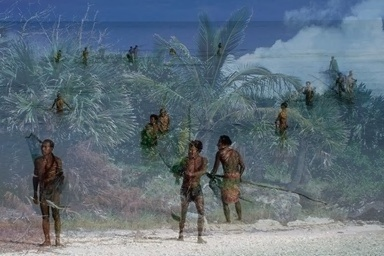
\includegraphics[width=0.245\linewidth]{\detokenize {figuras/gerada-3_blend.jpg}}&
%    % 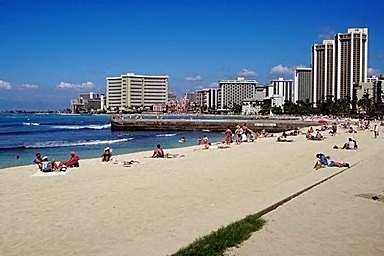
\includegraphics[width=0.19\linewidth]{\detokenize {figuras/gerada-4_unsharpMask.jpg}}&
%    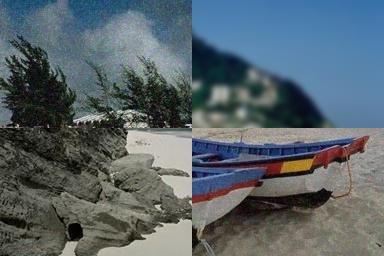
\includegraphics[width=0.245\linewidth]{\detokenize {figuras/gerada-5.jpg}} \\
%  \end{tabular}
%  \end{center}
%   \caption[Geração de imagens artificiais para o rebalanceamento de classes.]{Geração de imagens artificiais para o rebalanceamento de classes. A partir das imagens originais mostradas na primeira linha, são geradas imagens artificiais por meio de: borramento, adição de ruído, mistura e combinação. Os resultados dessas operações estão demonstrados na segunda linha, em ordem. \textit{Fonte:~Elaborado pela autora.}}
%  \label{fig:ArtificialImages}
% \end{figure}
% \renewcommand{\tabcolsep}{0.5cm}
% \vspace{25pt}
%
%
% Os descritores de características utilizados para os resultados foram apresentados na Seção \ref{sec:extracao}. \todo{qual experimento anterior? explicar!} Considerando que em um experimento anterior o melhor resultado foi atribuído à quantização com o método de Intensidade para o extrator Haralick e MSB para os outros, apenas esses testes foram aprofundados (tópico anteriormente discutido na Seção \ref{sec:quantizacao}). Neste experimento, o classificador KNN foi utilizado, com $K=1$. Inicialmente o classificador Naive Bayes foi explorado, apresentando melhora na acurácia ao apenas replicar as imagens. Esse comportamento não é desejado em um classificador para a avaliação de rebalanceamento de classes. O código desenvolvido para esses resultados preliminares está disponível em \url{https://bitbucket.org/moacirponti/imagefeatureextraction/overview}.
%
%
% %--------------------------------------------------------------------------------
% \subsection{Fluxo de operações}
%
% Para a realização desse experimento, iniciou-se com uma base originalmente balanceada e foram realizadas as seguintes operações:
%
% \begin{enumerate}
% \item Diminuir logaritmicamente o número de imagens de uma das classes, de modo a obter uma base desbalanceada;
% \item Para cada estágio de desbalanceamento, realizar três experimentos:
% \begin{enumerate}
% \item A classificação direta, sem nenhuma operação de rebalanceamento;
% \item A operação de SMOTE, após a extração de características e antes da classificação;
% \item Rebalanceamento da classe minoritária com a geração de imagens antes da extração de características.
% \label{item}
% \end{enumerate}
% \item Extrair as características com os descritores: ACC, BIC, CCV, GCH e Haralick6; e os quantizadores: Intensidade, Gleam, Luminância e MSB;
% \item Classificar com KNN utilizando validação cruzada por \textit{repeated random-subsampling};
% \item Executar os passos de 2 a 4 no mínimo 10 vezes para cada par de extrator e quantizador;
% \item Calcular a matriz de confusão, a acurácia balanceada, a medida-F e o teste de Friedman para os resultados encontrados;
% \item Gerar os gráficos para visualização dos resultados.
% \end{enumerate}
%
% %--------------------------------------------------------------------------------
% \subsection{Geração das imagens artificiais}
%
% As etapas para a geração das imagens artificiais, passo \ref{item} da seção anterior, foram:
%
% \begin{enumerate}
% \item Particionar a classe minoritária em conjuntos de treino e teste;
% \item Selecionar uma imagem aleatoriamente do conjunto de treino;
% \item Selecionar uma operação aleatória entre: borramento, adição de ruído, \textit{unsharp mask}, mistura ou composição;
% \begin{enumerate}
% \item Caso seja selecionada a composição: encontrar uma outra imagem aleatória, selecionar um quadrante dessa imagem e novamente uma operação entre: borramento, adição de ruído, \textit{unsharp mask} ou mistura;
% \end{enumerate}
% \item Aplicar essa operação na imagem previamente selecionada e adicionar essa imagem gerada ao conjunto de treino;
% \item Repetir os passos 2 a 4 até que as classes estejam igualmente balanceadas.
% \end{enumerate}
%
% %--------------------------------------------------------------------------------
% \section{Resultados}
% \label{sec:resultadospreliminares}
%
% Este estudo preliminar apresentou evidências experimentais de que, em problemas de duas classes (apresentadas na Figura~\ref{fig:praiamontanha}), pode haver ganho estatístico da medida-F ao gerar imagens, quando comparado à geração de exemplos artificiais no espaço de atributos (ou seja, depois que as características já foram extraídas das imagens). Essa melhoria pode ser notada na Figura~\ref{fig:resultmelhor}, que apresenta a relação da medida-F com a taxa de balanceamento, utilizando: as imagens originais, a geração de exemplos com SMOTE e as imagens geradas. Para essa configuração, foi utilizado o descritor de características ACC com a conversão em escala de cinza por MSB e a operação de pré-processamento por combinação. As classes ``praia'' e ``montanha'' foram escolhidas por serem as classes que possuem maior dificuldade de diferenciação, havendo alta taxa de sobreposição de intensidades de cores e texturas, conforme testes realizados.
%
% \vspace{20pt}
%
% \begin{figure}[!htb]
%  \begin{center}
%    \includegraphics[width=\linewidth]{\detokenize {figuras/praia-montanha.png}}
%  \end{center}
%   \caption[Classes ``praia'' e ``montanha'' da base de imagens COREL-1000.]{Classes ``praia'' (primeira linha) e ``montanha'' (segunda linha) da base de imagens COREL-1000. \textit{Fonte:~Elaborado pela autora.}}
%  \label{fig:praiamontanha}
% \end{figure}
%
% \vspace{10pt}
%
% \begin{figure}[!hbpt]
%  \begin{center}
% \begin{subfigure}{\textwidth}
%   \centering
%   \includegraphics[width=\linewidth]{\detokenize {figuras/resultado-melhor4.png}}
%   \caption{Original}
% \end{subfigure}
% \begin{subfigure}{\textwidth}
%   \centering
%   \includegraphics[width=\linewidth]{\detokenize {figuras/resultado-pior1.png}}
%   \caption{\textit{Unsharp masking}}
%   \label{fig:unsharp}
% \end{subfigure}
%  \end{center}
% \end{figure}
%
% \begin{figure}[htb]
%  \begin{center}
%    \includegraphics[width=\linewidth]{\detokenize {figuras/resultado-melhor4.png}}
%  \end{center}
%  \caption[Resultado obtido com a operação de combinação apresentada na Figura~\ref{fig:ArtificialImages}.]{Resultado obtido com a operação de combinação apresentada na Figura~\ref{fig:ArtificialImages}. Apresenta-se a relação da medida-F com a taxa de balanceamento utilizando: as imagens originais, a geração de exemplos com SMOTE e as imagens geradas artificialmente. \textit{Fonte:~Elaborado pela autora.}}
%  \label{fig:resultmelhor}
% \end{figure}
%
% \enlargethispage{-1cm}
%
% Também foi possível notar que algumas operações não provocaram a melhora da classificação. A operação de adição de ruído para geração artificial, a posterior extração utilizando CCV e a quantização por MSB, destacou-se como o pior resultado, apresentado na Figura~\ref{fig:resultpior}. Outros casos que não obtiveram o resultado esperado envolveram as operações de borramento e de \textit{unsharp masking}.
%
% \begin{figure}[htb]
%  \begin{center}
%    \includegraphics[width=\linewidth]{\detokenize {figuras/resultado-pior1.png}}
%  \end{center}
%  \caption[Piores resultados, obtidos com a adição de ruído.]{Piores resultados, obtidos com a adição de ruído. Apresenta-se a relação da medida-F com a taxa de balanceamento utilizando as imagens originais, o SMOTE e as imagens artificiais geradas. \textit{Fonte:~Elaborado pela autora.}}
%  \label{fig:resultpior}
% \end{figure}
%
% Após a realização dos testes, as operações que melhor se destacaram foram: utilizar todas as operações, apenas mistura e apenas composição. E as operações que resultaram em uma classificação pior do que o uso do SMOTE foram: utilizar apenas borramento, ruído ou \textit{unsharp masking}. Com o teste estatístico de Friedman foi possível verificar que o ACC foi o extrator que melhor se beneficiou das características geradas; e CCV e GCH os menos beneficiados. \enlargethispage{-\baselineskip} A Tabela \ref{tab:result} apresenta os \textit{rankings} encontrados por este teste para todas as execuções das melhores operações. O p-valor computado corresponde a $4.24E^{-11}$, assim a hipótese nula de que não há diferença entre as execuções foi rejeitada. Vale destacar que para algumas execuções, o teste de Friedman retornou o \textit{ranking}: geração artificial (1), SMOTE (2) e imagens originais (3), ou seja, sem que SMOTE e a geração artificial concorressem pela mesma posição, diferente da tabela apresentada.
%
% \begin{table}[htb]
% \centering
% \caption{Posição média dos algoritmos utilizando Friedman}
%   \begin{tabular}{c|c}
%     Algoritmos  &   Posição \\ \hline
%     Original    &   3.0000  \\
%     Smote       &   1.6136  \\
%     Artificial  &   1.3863  \\
%   \end{tabular}
%  \label{tab:result}
% \end{table}
%
% Em outro experimento, utilizou-se as cópias das imagens de treino para rebalancear, sem realizar nenhuma operação de pré-processamento (método conhecido como SRS - \textit{Simple Random Sampling}). A Figura~\ref{fig:resultcopia} mostra as respectivas medidas-F encontradas. É possível notar que a cópia dessas imagens não adiciona nenhuma informação nova para o aprendizado.
%
% \begin{figure}[htb]
%  \begin{center}
%    \includegraphics[width=\linewidth]{\detokenize {figuras/resultado-copia.png}}
%  \end{center}
%   \caption[Simples replicação de exemplos sem realizar nenhuma operação.]{Simples replicação de exemplos sem realizar nenhuma operação de pré-processamento. É possível verificar que não foi adicionada nenhuma informação relevante para o aprendizado. \textit{Fonte:~Elaborado pela autora.}}
%  \label{fig:resultcopia}
% \end{figure}
%
%
\section{Considerações Finais}

% Com os experimentos realizados foi possível notar que a geração de imagens artificiais pode gerar novas informações para a classificação das imagens. O que indica que um estudo mais aprofundado de quais operações podem ser aplicadas nas imagens originais auxilie o cenário de bases desbalanceadas.
%
% Dessa forma, esse capítulo também apresentou as próximas tarefas a serem realizadas. Foi destacada a análise das redes de convolução para identificar quais características latentes são automaticamente extraídas. Apesar de algumas operações de pré-processamento terem gerado imagens que melhoraram a classificação, algumas não causaram melhora. Isso indica que a análise da relevância da informação contida em imagens deve melhorar esse resultado. A memória associativa, aprendida com uma máquina de Boltzmann restrita, deve ser capaz de indicar se uma determinada imagem é relevante para o aprendizado.
